\documentclass[11pt,ngerman]{scrartcl}

% standard packages
\usepackage[utf8]{inputenc}  % input in UTF-8
\usepackage[T1]{fontenc}  % output in T1 fonts (westeuropäische Codierung)
\usepackage{lmodern}  % latin modern fonts
\usepackage[ngerman]{babel}  % deutsches Sprachpaket, neue Rechtschreibung

% Seitensetup
\usepackage{scrlayer-scrpage}  % Seitenformatierung durch KOMA-interne Optionen
\usepackage[top=4cm, bottom=4cm]{geometry}  % Seitengeometrie (kann durch KOMA ersetzt werden, hab ich aber nicht geschafft)
\usepackage[hypcap=false]{caption, subcaption}  % caption editing - hypcap warning with hyperref
\usepackage{array}  % table editing

% additional packages
\usepackage{amsmath, amssymb, amstext}  % math packages (American Math Society)
\usepackage{bm}
\usepackage{icomma}  % Kommata in Dezimalzahlen verursachen keinen Abstand mehr
\usepackage{graphicx}  % Bilder einfügen
\usepackage{float} %Bilder placement
\usepackage{pdfpages}  % PDF als vollständige Seiten einfügen
\usepackage{lastpage}  % referenziert die letzte Seite
\usepackage[separate-uncertainty=true]{siunitx}  % bessere Darstellung von Einheiten
\usepackage{makecell} %Dicke Tabellenstriche
\usepackage{longtable}
\usepackage{booktabs}
%\usepackage{datatool}
\usepackage[hidelinks]{hyperref}  % hyperref verlinkt Referenzen - hidelinks entfernt borders um links

% package setups
% Kopf- und Fußzeile durch KOMA
\pagestyle{scrheadings}  % KOMA darf entscheiden
\clearpairofpagestyles  % reset
\setkomafont{pageheadfoot}{\normalfont}  % Standardschrift in Kopf- und Fußzeile
\captionsetup{format=plain, font=small, labelfont=bf} %Better caption, Abbildung ist FETT
%\setlength{\headheight}{27.2pt}  % benötigte Höhe Kopfzeile (warning von scrlayer-scrpage, wird aber automatisch so gerendert, falls diese Option weggelassen wird)
\ihead{Oszillograph}  % Kopf links %Todo Titel ändern
\chead{\textsc{Philipp} Maximilian \\ \textsc{Stark} Matthias}  % Kopf Mitte %Todo Name ändern
\ohead{10 Dezember 2021}  % Kopf rechts %Todo Datum ändern
\cfoot{\pagemark \, / \pageref{LastPage}}  % Fuß Mitte

% Table of Contents
\DeclareTOCStyleEntry{dottedtocline}{section}  % KOMA intern - Inhaltsverzeichnis mit Punkten (nur sections)

%Overbar setup
\newcommand{\overbar}[1]{\mkern 1.5mu\overline{\mkern-1.5mu#1\mkern-1.5mu}\mkern 1.5mu}
% SI
\sisetup{locale = DE}  % deutschsprachige SI-Konvention
\sisetup{quotient-mode = fraction}
\sisetup{per-mode = fraction}
\DeclareSIUnit\px{px}
\DeclareSIUnit\strich{|||}
\DeclareSIUnit\mF{$\mu$F}

% citation
\usepackage{csquotes}
%\usepackage[backend=biber]{biblatex}
\usepackage[backend=biber]{biblatex}
\addbibresource{oszi.bib} %Todo .bib befüllen zb.: mit JabRef (Empfehlung der Redaktion)

%Eigene Commands
\newcommand{\der}[2]{\frac{\mathrm{d}#1}{\mathrm{d}#2}}
\newcommand{\pder}[2]{\frac{\partial #1}{\partial #2}}

%\noindent für ges
\setlength{\parindent}{0pt}


\begin{document}
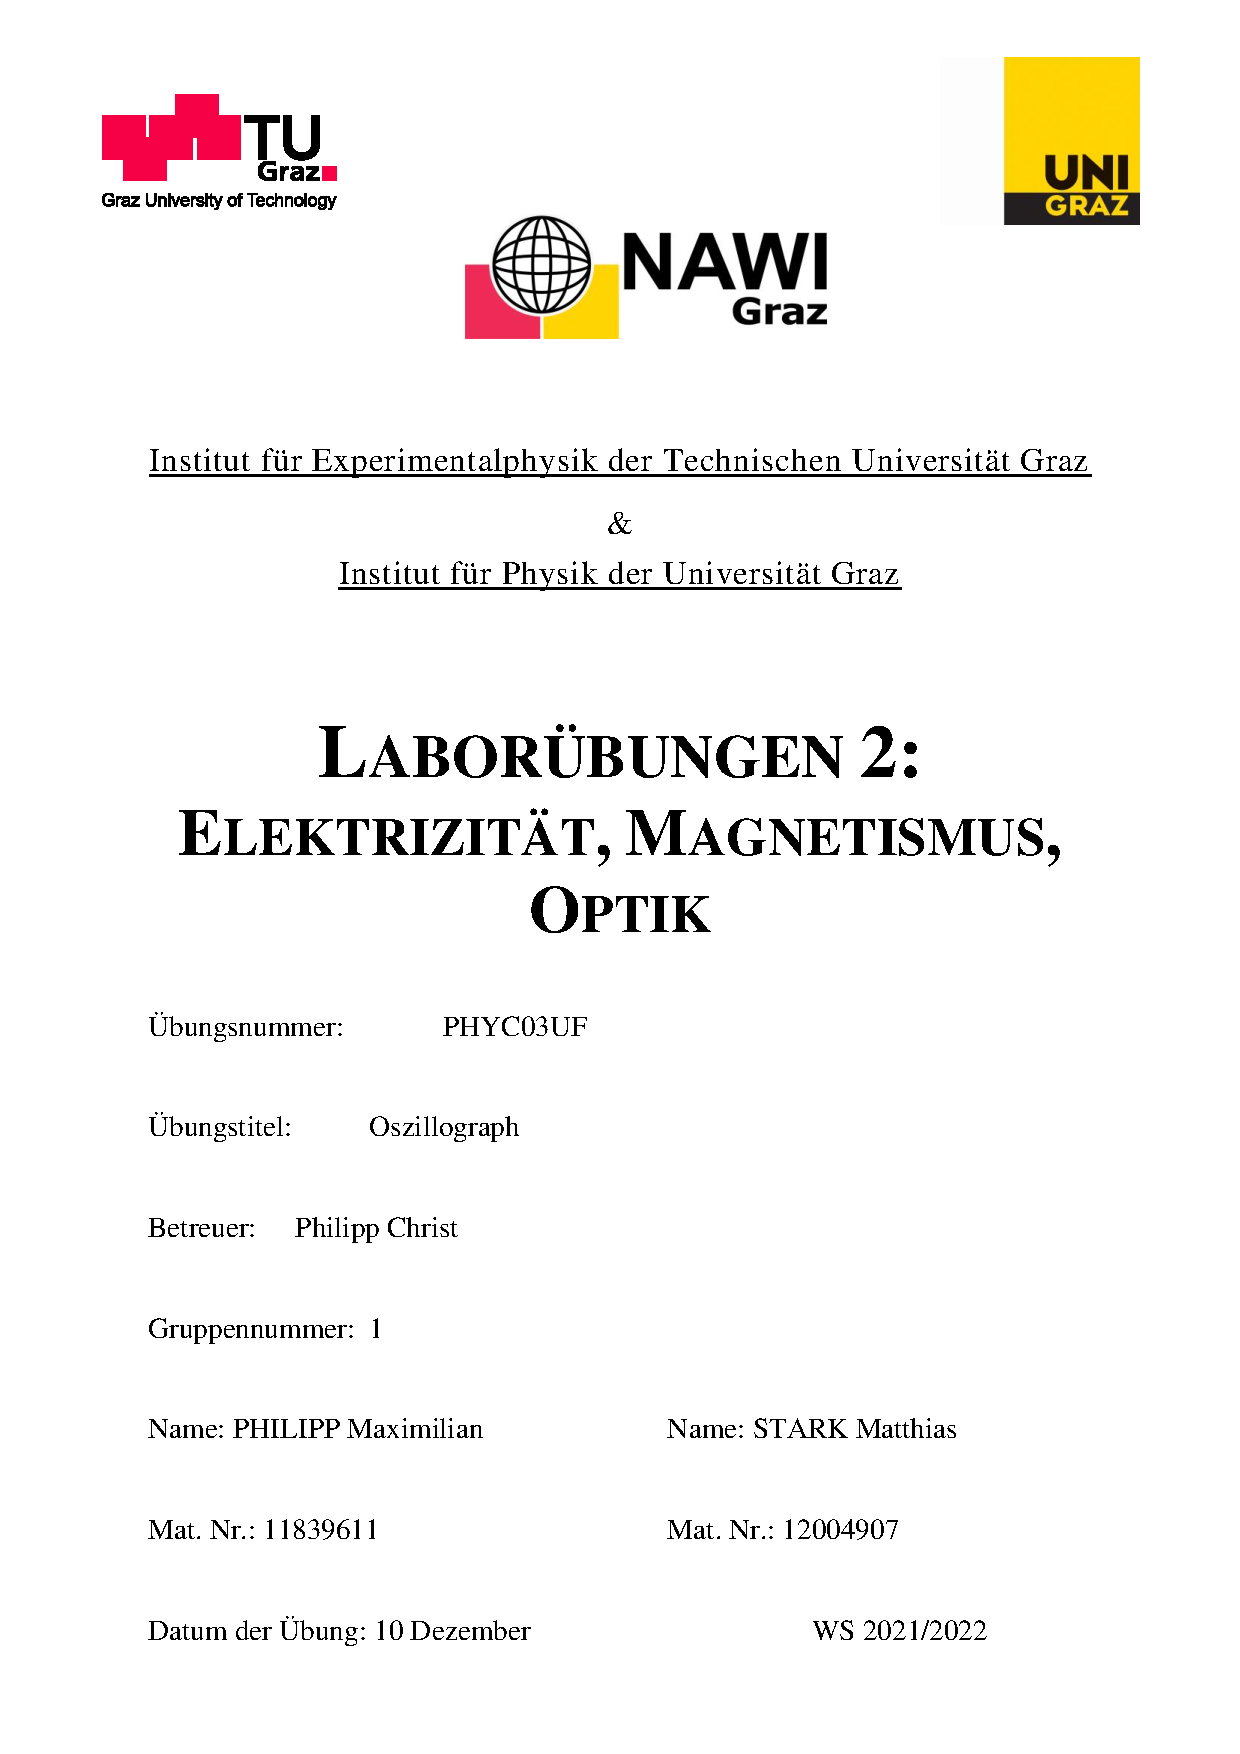
\includepdf{Deckblatt_labor2.pdf}
\tableofcontents
\newpage

\section{Aufgabenstellung\label{Auf0}}

\begin{itemize}
	\item Kennenlernen des Kathodenstrahloszilloskops. Stellen Sie einige Lissajous-Figuren auf dem
	      Kathodenstrahloszilloskop dar. Beschreiben Sie kurz, wie damit grob der Frequenzunterschied
	      von zwei Signalen ermittelt werden kann. Gehen Sie dazu wie folgt vor:
	      \begin{itemize}

		      \item Schließen sie je einen Funktionsgenerator an je einen Kanal des Oszilloskops an.

		      \item Stellen Sie eine feste Frequenz an einem der beiden Funktionsgeneratoren ein.

		      \item Verändern sie jetzt die Frequenz am anderen Funktionsgenerator und beobachten sie den Schirm des Oszilloskops.

		      \item Wann bekommen sie ein stehendes Bild? Wann entstehen Kreuzungspunkte?

	      \end{itemize}

	\item Bauen Sie eine Serienschaltung aus einem ohm’schen Widerstand ($R =$ \SI{200}{\kilo\ohm}) und einer
	      Kapazität $(C =$ \SI{1}{\micro\farad}) auf. Verwenden Sie für die folgenden Unterpunkte das digitale
	      Oszilloskop. Lesen sie die Messdaten über den PC ein und stellen sie Strom und Spannung
	      am Kondensator über der Zeit dar. Untersuchen Sie den zeitlichen Verlauf von Strom und
	      Spannung am Kondensator für:

	      \begin{itemize}

		      \item eine sinusförmige Speisespannung von \SI{50(1)}{\hertz}

		      \item eine rechteckförmige Speisespannung von \SI{50(1)}{\hertz}

		      \item Bestimmung der Abklingzeit für den Fall der rechteckförmigen Speisespannung von
		            \SI{50(1)}{\hertz}: Exportieren Sie den Spannungsabfall über den PC und plotten ihn mit Hilfe
		            eines Datenanalyseprogramms. Fitten Sie die Funktion und bestimmen
		            Sie so die Zerfallskonstante. Überprüfen Sie Ihr Ergebnis durch vergleichen mit
		            dem zu erwartenden Wert für $\tau = R C$.

	      \end{itemize}

	      Erklären Sie die Ergebnisse.

	\item Bauen Sie einen Serienschwingkreis nach \autoref{fig:abb6} mit $R = $ \SI{200}{\ohm} und $C = $ \SI{1}{\micro\farad} auf. Als Induktivität verwenden sie zwei in Serie geschaltete Spulen ($n=500$) mit beweglichem Eisenkern. Zeichnen Sie mit dem digitalen Oszilloskop die folgenden Fälle des Serienschwingkreis
	      bei \SI{50(1)}{\hertz} auf:

	      \begin{itemize}

		      \item Kriechfall

		      \item Aperiodischer Grenzfall

		      \item Schwingfall

	      \end{itemize}
	      Sie können durch verschieben des Eisenkerns in der Spule die Induktivität verändern und
	      wechseln so zwischen den oben angeführten Fällen.

\end{itemize}

\newpage

\section{Grundlagen}

\subsection{Aufbau eines Kathodenstrahloszilloskops}

Ein Oszilloskop dient im allgemeinen zur Darstellung zeitlicher Verläufe von elektrischen Spannungssignalen.
Die Auslenkung am Schirm ist dabei der angelegten Spannung proportional.
Sollen andere physikalische Größen dargestellt werden, so sind entsprechende Wandler notwendig.

In der Braun’schen Röhre des Kathodenstrahloszilloskops (siehe \autoref{fig:abb1}) werden von der geheizten
Kathode $K$ Elektronen emittiert und gegen die Anode $A$ hin beschleunigt. Durch eine Öffnung können die Elektronen diese durchsetzen. Durch die an die Horizontal- $P_x$ bzw. Vertikalablenkplatten $P_y$ angelegten Spannungen $U_x$ bzw. $U_y$ werden sie abgelenkt, und treffen auf den Leuchtschirm $L_S$.

\begin{figure}[H]
	\begin{center}
		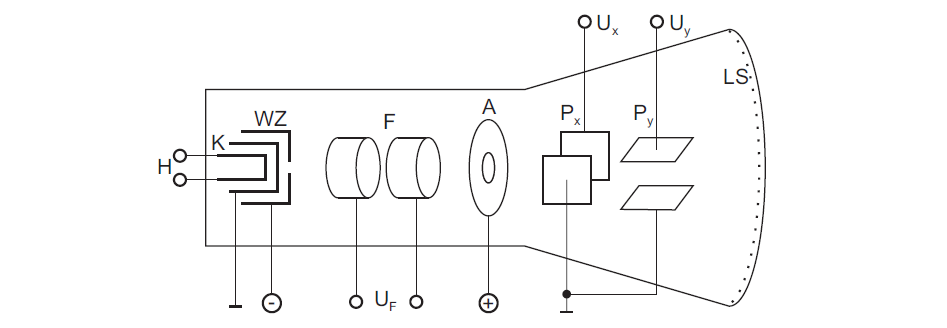
\includegraphics[width=\textwidth]{abb1}
	\end{center}
	\caption{Schematische Darstellung einer Braun’schen Röhre. $H$ Heizdraht; $K$ Kathode; $WZ$
		Wehnelt-Zylinder; $F$ Fokussierelektroden; $U_F$ Fokussierspannung; $A$ Anode; $P_x$, $P_y$ Platten für
		Horizontal- und Vertikalablenkung; $U_x$, $U_y$ Spannungen für horizontale und vertikale Ablenkung;
		$LS$ Schirm mit Leuchtstoff.}
	\label{fig:abb1}
\end{figure}

Um die Stärke des Elektronenstrahls und somit die Helligkeit des Bildes zu regeln, kann die
negative Spannung am Wehnelt-Zylinder $WZ$ variiert werden. Damit können diesen nur Elektronen
mit einer hinreichend großen Energie verlassen. Zur Fokussierung des Strahls werden
meist elektrische Linsen $F$ verwendet. Die notwendige Fokussierspannung $U_F$ ist unter anderem
von der Intensität des Elektronenstrahls abhängig.

Das Blockschaltbild eines einfachen, triggerbaren (s. \autoref{sec:1_2}) Zweikanal-Oszilloskops ist in
\autoref{fig:abb2} zu sehen. Die an den Kanälen 1 und 2 anliegenden Spannungen können gefiltert und
verstärkt, sowie in der Position verschoben werden. Im AC-Betrieb ist, anders als im DC-Mode,
der Kondensator (s. \autoref{fig:abb2}) nicht durch den Schalter kurzgeschlossen, weshalb die Nulllinie am
Oszilloskop der Zeitmittelwert der untersuchten Spannung ist. Zu beachten ist der Spannungsabfall von
zwar rein periodischen Spannungen mit niedriger Frequenz. Hier kann es zu Verzerrungen im
AC-Modus kommen (Versuch: Rechtecksignal bei \SI{50(1)}{\hertz}).

\begin{figure}[H]
	\begin{center}
		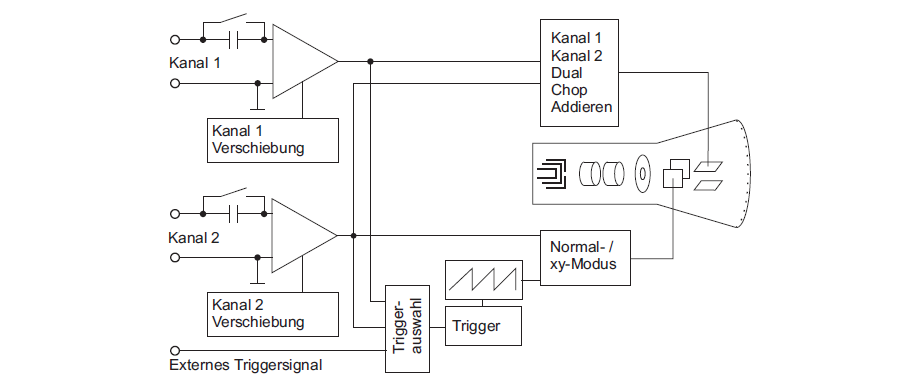
\includegraphics[width=\textwidth]{abb2}
	\end{center}
	\caption{Blockschaltbild eines einfachen triggerbaren Zweikanal-Oszilloskops}
	\label{fig:abb2}
\end{figure}

Im Normalbetrieb kann gewählt werden, ob nur ein Kanal oder beide angezeigt werden. Auch eine
Addition der Kanäle ist möglich. In diesen Betriebsarten liegt an den horizontalen Ablenkplatten
eine Sägezahnspannung an, die über einen Trigger angesteuert wird.

Im xy-Modus liegt Kanal 1 an der y-Ablenkung, Kanal 2 an der x-Ablenkung. Sägezahn sowie
Triggerung sind in diesem Modus unbenutzt.



\subsection{Normalbetrieb, Triggerung}\label{sec:1_2}

An die Horizontalablenkung wird eine Sägezahnspannung gelegt, das heißt, der Kathodenstrahl
wird mit konstanter Geschwindigkeit über den Schirm bewegt. Ist er am rechten Rand angekommen,
so wird er rasch an den linken zurückbewegt. In dieser Zeit wird der Elektronenstrahl
abgeschaltet. Wird ohne Triggerung gearbeitet, so startet der Sägezahn sofort wieder (dies ist
beim Hameg HM 203-6 Oszilloskop z.B. dann der Fall, wenn im automatischen Triggermodus
kein Triggerpuls gefunden wird).

An der y-Ablenkung liegt im Einkanal-Betrieb einer der beiden Kanäle an. Im Zweikanal-Betrieb
wird zuerst der eine Kanal ganz gezeichnet, mit dem nächsten Sägezahnpuls der andere. Bei sehr
langsamen Signalen führt dies zu einem störenden Flackern der Messkurven. In diesem Fall kann
auf Chop-Betrieb umgestellt werden, d.h. während eines Sägezahnpulses werden wechselweise
Kanal 1 und 2 dargestellt.

Um für periodisch wiederkehrende Signale ein stehendes Bild zu erhalten, wird in den heute
üblichen Oszilloskopen die Triggerung verwendet (vgl. \autoref{fig:abb3}). Die Spannung an der Horizontalablenkung
wird so gewählt, dass sich der Elektronenstrahl am linken Schirmrand befindet,
die Intensität ist Null (Ruhestellung). Über- bzw. unterschreitet die Triggerspannung $U_y$ einen
vorgegebenen Wert (Triggerlevel), so startet der Sägezahn und das Signal wird auf den Schirm
geschrieben. Ist der Strahl am rechten Rand angelangt, so kehrt er in die Ruhestellung zurück
und wartet auf den nächsten Triggerpuls.

Bei älteren Geräten wurde ein stehendes Bild dadurch erzeugt, dass die Periodendauer des Sägezahns
mit jener des Signals synchronisiert wurde.

Zur Darstellung nicht periodischer Signale werden Speicheroszilloskope verwendet. Dabei wird
das zu untersuchende Signal zwischengespeichert und der Inhalt des Speichers am Schirm angezeigt.

\vspace{2mm}

\begin{minipage}{\textwidth}
	\begin{minipage}[t]{0.66\textwidth}
		\centering
		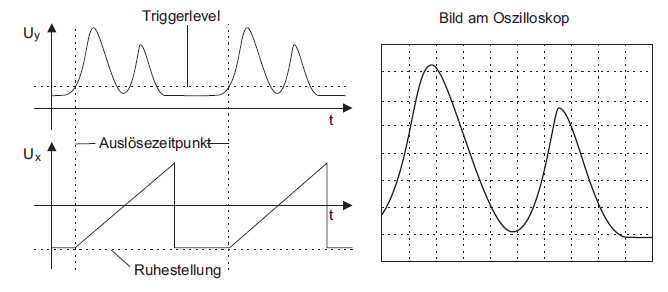
\includegraphics[width=\textwidth]{abb3}
		\captionbelowof{figure}{Triggerung: $U_y$ zu messendes Signal, dient hier
			gleichzeitig zur Triggerung; $U_x$ von Trigger und Sägezahngenerator
			erzeugte Spannung für Horizontalablenkung.}
		\label{fig:abb3}
	\end{minipage}
	\vspace{2mm}
	\begin{minipage}[t]{0.33\textwidth}
		\centering
		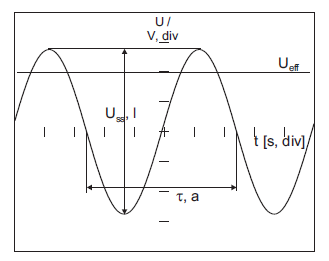
\includegraphics[width=\textwidth]{abb4}
		\captionof{figure}{Kalibrierung des
			Spannungs- bzw. Zeitablenkfaktors.}
		\label{fig:abb4}
	\end{minipage}
	\vspace{1em}
\end{minipage}

\subsection{xy - Betrieb}

Der xy-Betrieb des Kathodenstrahloskilloskops wird zur Darstellung von funktionalen Abhängigkeiten
zwischen zwei zeitabhängigen Größen $U_x \hat{=} x(t)$ und $U_y \hat{=} y(t)$ verwendet. Dabei wird
$U_y$ an die Vertikalablenkung (Kanal 1) und $U_x$ an die Horizontalablenkung (Kanal 2) gelegt, am
Schirm wird damit $y = f(x)$ dargestellt.

Eine Anwendung ist die Darstellung von Kennlinien elektrischer Bauelemente, vgl. Praktikumsübung
``Halbleiterdiode``. Weiters können unter Zuhilfenahme von Lissajou-Figuren die
Frequenzen zweier Signale angeglichen bzw. Frequenzverhältnisse gemessen werden. Auch die
Bestimmung von kleinen Phasenverschiebungen zwischen zwei Signalen ist so möglich.

Werden im xy-Betrieb beide Kanäle gleichzeitig auf Erdpotential gelegt, so ist nur mehr ein
Punkt am Bildschirm zu sehen. Diese Einstellung sollte vermieden werden, weil der Fluoreszenzbelag
durch andauernde Bestrahlung zerstört werden kann.

\subsection{Wandler}

Sollen andere Größen als Spannungen am Oszilloskop gemessen werden, so müssen diese in
Spannungen umgewandelt werden. Zur Messung von elektrischen Strömen werden ohm’sche
Widerstände als Wandler verwendet, für Temperaturen z.B. Thermoelemente, für Magnetfelder
Hallsonden, etc. Die Bestimmung der jeweiligen Ablenkfaktoren (z.B. A/cm) kann entweder
durch das Anlegen bekannter Signale oder die Ausnutzung physikalischer Zusammenhänge im
Wandler (z.B. $U = RI$) geschehen.


\newpage

\section{Versuchsanordnung}\label{sec:Versuchsanordnung}

Zur Bestimmung des zeitlichen Verlaufs von Strom und Spannung an einem Kondensator wird ein
Aufbau nach \autoref{fig:abb5} verwendet. Ein spezieller Trenntrafo $T$ dient zur Trennung des erdbehafteten
Signals aus $F$ von der Erde. Dennoch ist zu beachten, dass Erdschleifen über das Oszilloskop
vermieden werden.

\begin{figure}[H]
	\begin{center}
		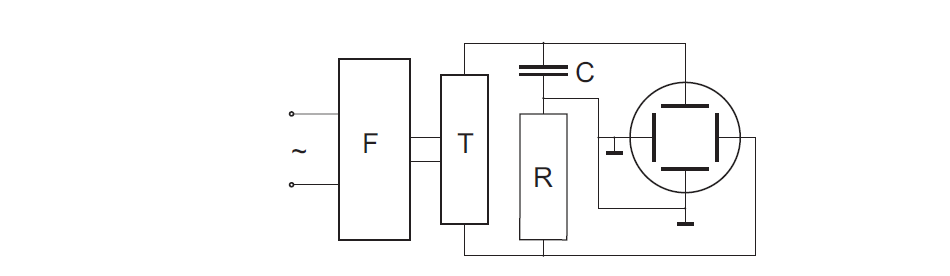
\includegraphics[width=\textwidth]{abb5}
	\end{center}
	\caption{Aufbau zur Messung des zeitlichen Verlaufs von Strom und Spannung an einer Kapazität $C$.}
	\label{fig:abb5}
\end{figure}

Ein geschlossener Stromkreis, bestehend aus einer Kapazität, einer Induktivität und einem Widerstand,
stellt einen gedämpften elektrischen Schwingkreis dar (siehe \autoref{fig:abb6}). Im Falle eines
Serienschwingkreis gilt die Maschenregel:

\begin{equation}
	u_C + u_L + u_R = 0
\end{equation}

Setzt man $u_L = L\, di/dt, u_R = Ri$, folgt durch Differenzieren von Glg. 1 und mit $i_c = C \,du_c/dt$
die Differentialgleichung des Schwingkreises:

\begin{equation}
	\frac{d^2i}{dt^2} + \frac{R}{L} \frac{di}{dt} + i\frac{1}{LC} = 0
\end{equation}

Mit Hilfe der charakteristischen Gleichung (Glg. 3) können drei Fälle unterschieden werden.

\begin{itemize}

	\item 1. $R^2C - 4L > 0$: zwei reelle Lösungen $\Rightarrow$ Kriechfall

	\item 2. $R^2C - 4L = 0$: eine reelle doppelte Lösungen $\Rightarrow$ Aperiodischer Grenzfall

	\item 3. $R^2C - 4L < 0$: zwei imaginäre Lösungen $\Rightarrow$ Schwingfall

\end{itemize}

\begin{equation}
	\lambda^2 + \lambda \frac{R}{L} + \frac{1}{LC} = 0
\end{equation}

\begin{figure}[H]
	\begin{center}
		
\includegraphics[width=\textwidth]{abb6}
	\end{center}
	\caption{Serienschwingkreis}
	\label{fig:abb6}
\end{figure}

Im, in der Übung vorliegenden Fall, wird der Schwingkreis durch einen Frequenzgenerator als
Spannungsquelle periodisch mit einer rechteckförmigen Spannung angeregt. Es sollen die drei
unterschiedlichen Verhaltensweisen des Schwingkreises mit dem Oszilloskop aufgenommen werden.
Es wird sich zeigen, dass der Strom/Spannugsverlauf von den gewählten Bauteilgrößen
abhängen wird.



\section{Geräteliste}

\noindent Für die Messungen wurden folgende Geräte verwendet:

\captionof{table}{Verwendete Geräte }
\begin{center}
	\begin{tabular}{|c|c|c|c|} \hline
		\textbf{Gerät}        & \textbf{Typ}         & \textbf{Hersteller} \\ \hline
		Digitales Oszilloskop & DS1052E              & Rigol               \\ \hline
		Analoges Oszilloskop  & HM203-6              & Hameg               \\ \hline
		Computerprogramm      & Ultrascope           &                     \\ \hline
		Funktionsgenerator    & FG-5000 (VII/1287/1) & Wavetek             \\ \hline
		Trenntrafo            & 30 Vpp Max           &                     \\ \hline
		Widerstand            & \SI{1000}{\ohm}      &                     \\ \hline
		Widerstand            & \SI{200}{\ohm} (C6)  &                     \\ \hline
		Kondensator           & \SI{1}{\micro\farad} &                     \\ \hline
		4 Spulen              & 500 Windungen        &                     \\ \hline
		Eisenkerne            & E23 / VII/816/1      &                     \\ \hline
		Kabel                 & Bananenstecker       &                     \\ \hline
		Kabel                 & Koaxialanschluss     &                     \\ \hline
	\end{tabular}
\end{center}

\newpage

\section{Versuchsdurchführung \& Messergebnisse}\label{sec:Versuchsdurchführung}

\subsection{Kennenlernen des Kathodenstrahloszilloskops}

Dieser Teil des Versuchs wird vom Laborbetreuer durchgeführt, indem 2 Frequenzgeneratoren an das Kathodenstrahloszilloskop auf Kanal 1 und 2 angeschlossen werden. Nun werden die Frequenzen variiert und der Bildschirm des Oszilloskops betrachtet. Wird bei beiden Generatoren annähernd die Selbe Frequenz eingestellt, entsteht ein Kreis, welcher solange rotiert, bis die Frequenzen exakt gleich sind. An der Rotationsgeschwindigkeit kann bestimmt werden, wie weit entfernt die Frequenzen voneinander sind. Die erhaltenen Bilder werden ``Lissajou Figuren`` genannt.
Sind auf den beiden Kanälen nicht die selben Amplituden eingestellt, wird anstatt des Kreises eine Ellipse sichtbar, anhand deren Ausrichtung die Amplitudenverhältnisse bestimmt werden können.

\vspace{2mm}

Nun wird am 2. Frequenzgenerator eine deutlich größere Frequenz eingestellt. Handelt es sich dabei um ein Vielfaches des anderen Frequenz, so entstehen Knotenpunkte, wie beispielsweise für die Frequenzen von \SI{50}{\hertz} und \SI{200}{\hertz} in folgender \autoref{fig:lissajou} ersichtlich. Da 3 Knotenpunkte sichtbar werden handelt es sich um das Verhältnis 1:4, was sich auch mit den Werten deckt. Auch hier ergibt sich nur dann ein stehendes Bild, wenn die Frequenzen einem genauen Vielfachem entsprechen.

\begin{figure}[H]
	\begin{center}
		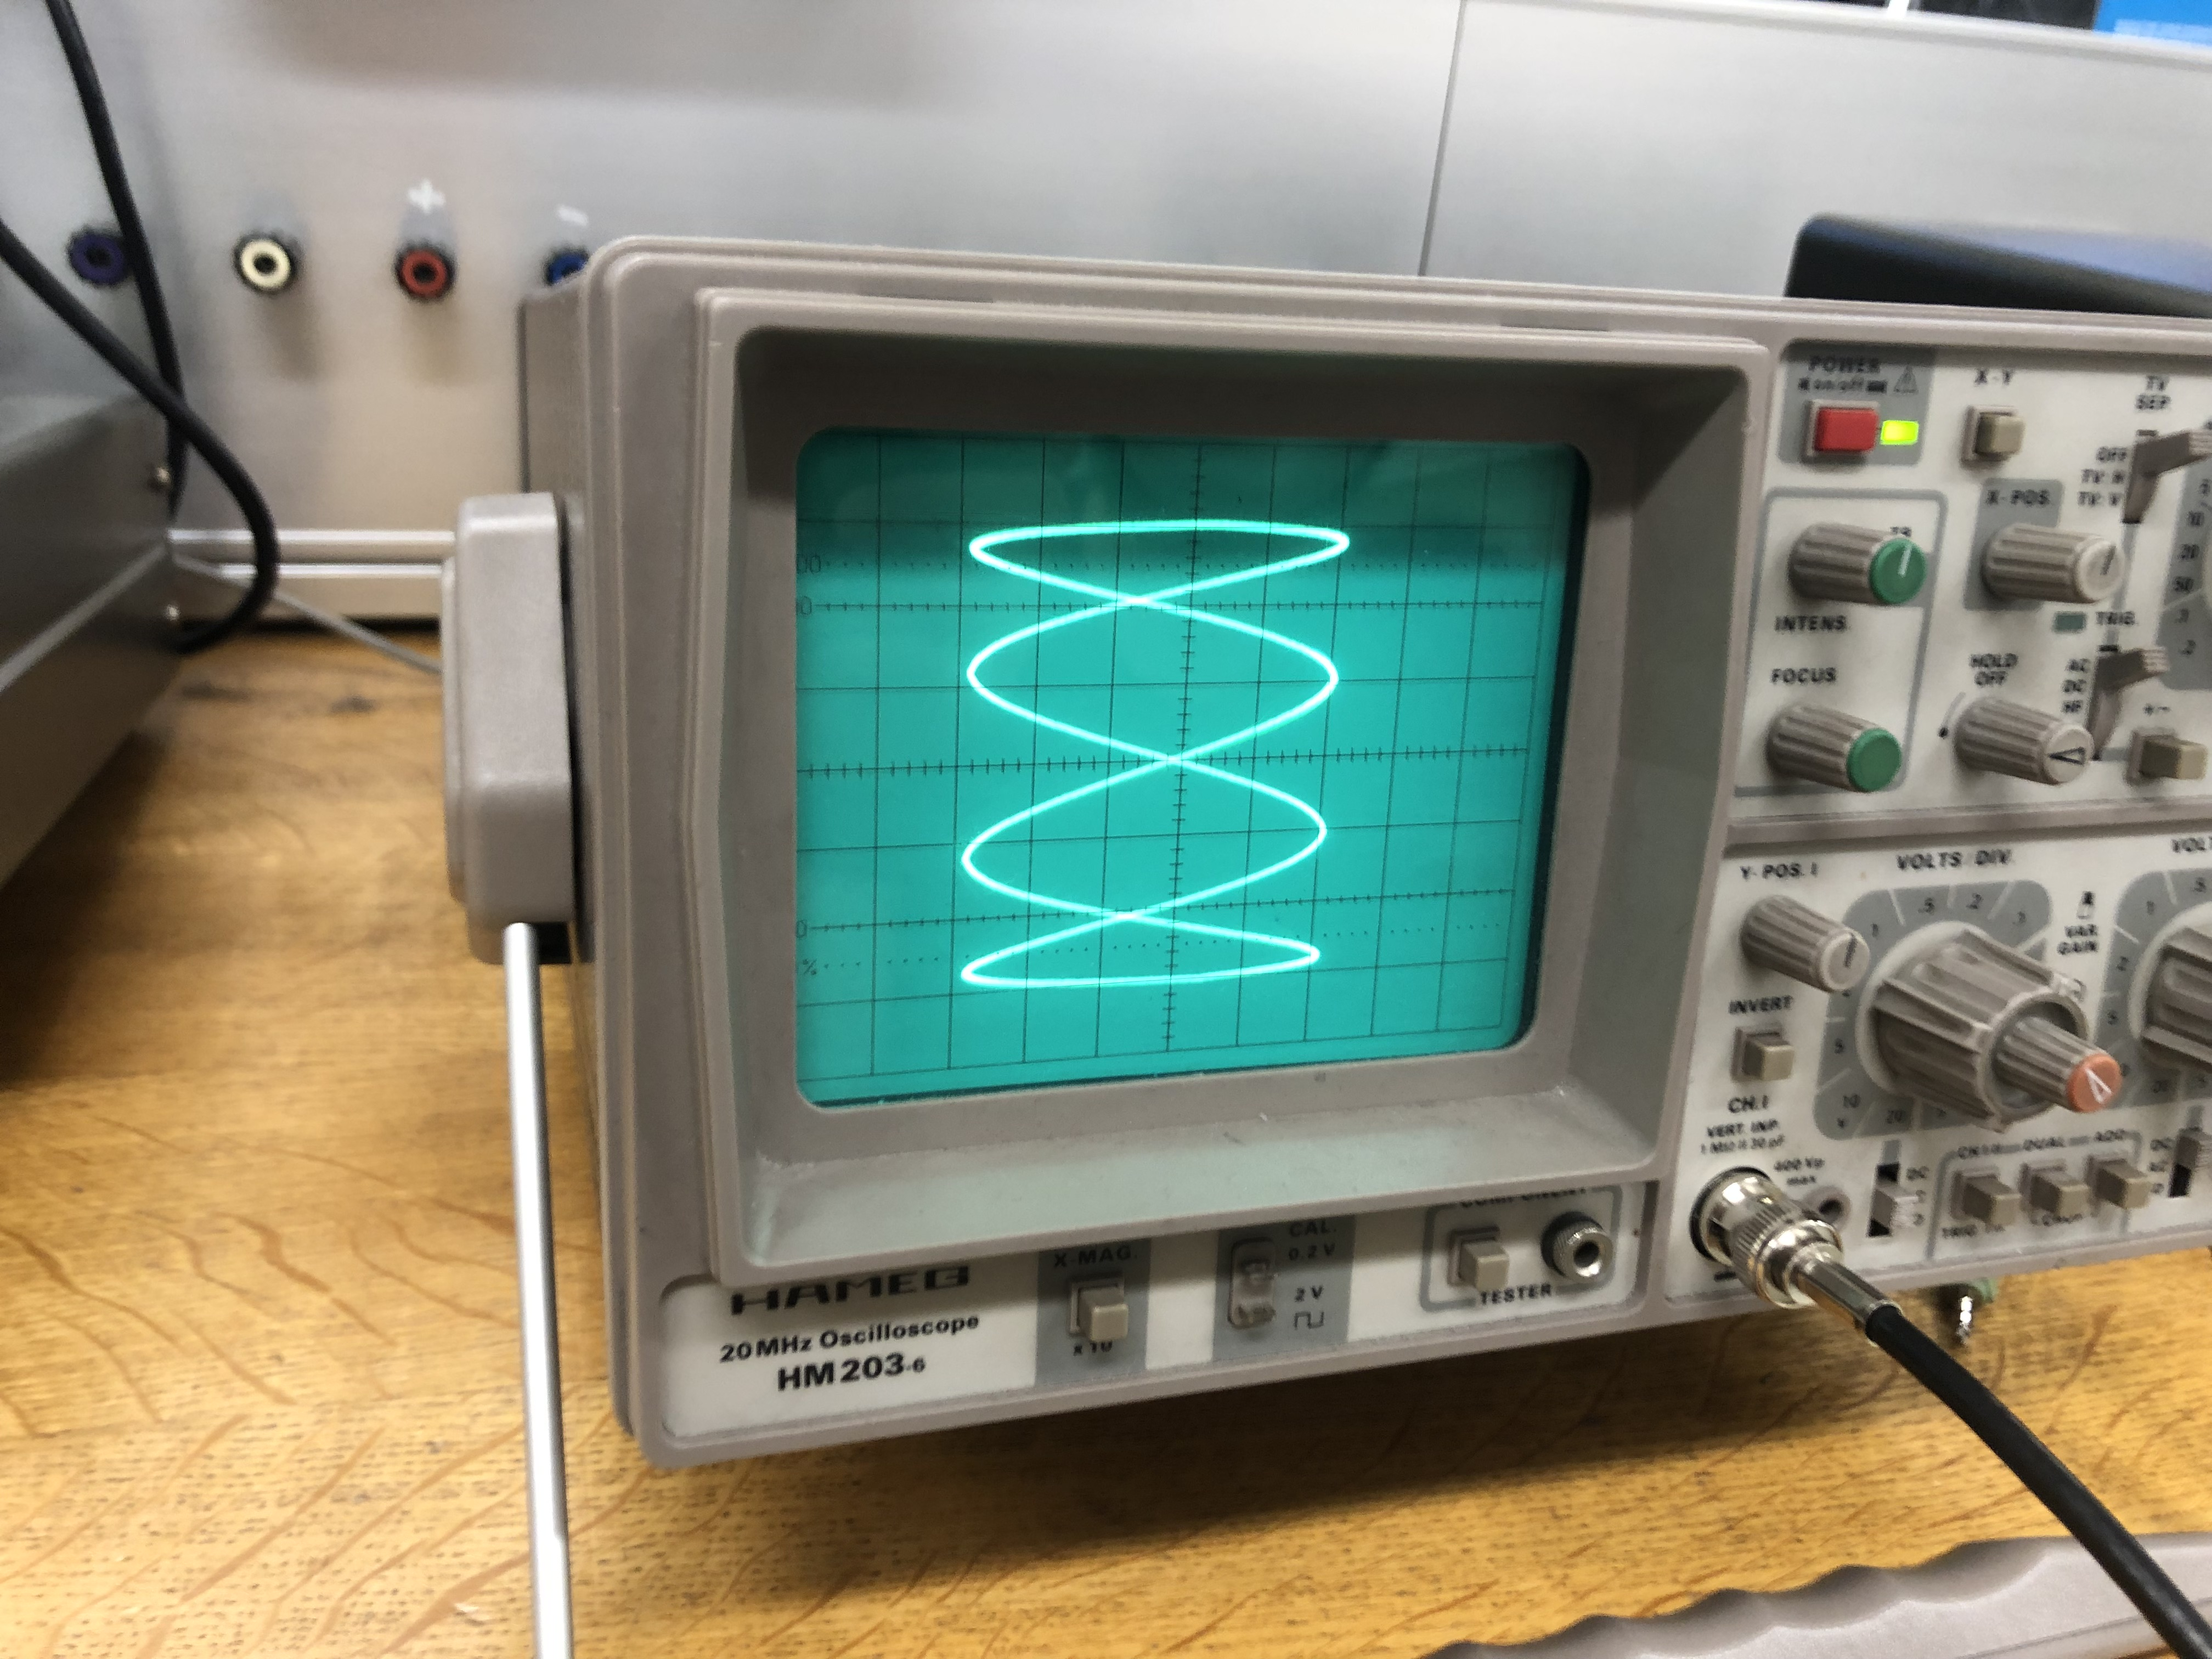
\includegraphics[width=0.7\textwidth]{figur}
	\end{center}
	\caption{Lissajou Figur mit 3 Knotenpunkten}
	\label{fig:lissajou}
\end{figure}

\newpage

\subsection{Serienschaltung aus ohm´schen Widerstand und Kapazität}

Der weitere Versuch wird mithilfe des digitalen Oszilloskops durchgeführt. Zunächst wird der Versuch nach der Skizze in \autoref{fig:abb5} aufgebaut, wodurch sich folgende Schaltung ergibt.

\begin{figure}[H]
	\begin{center}
		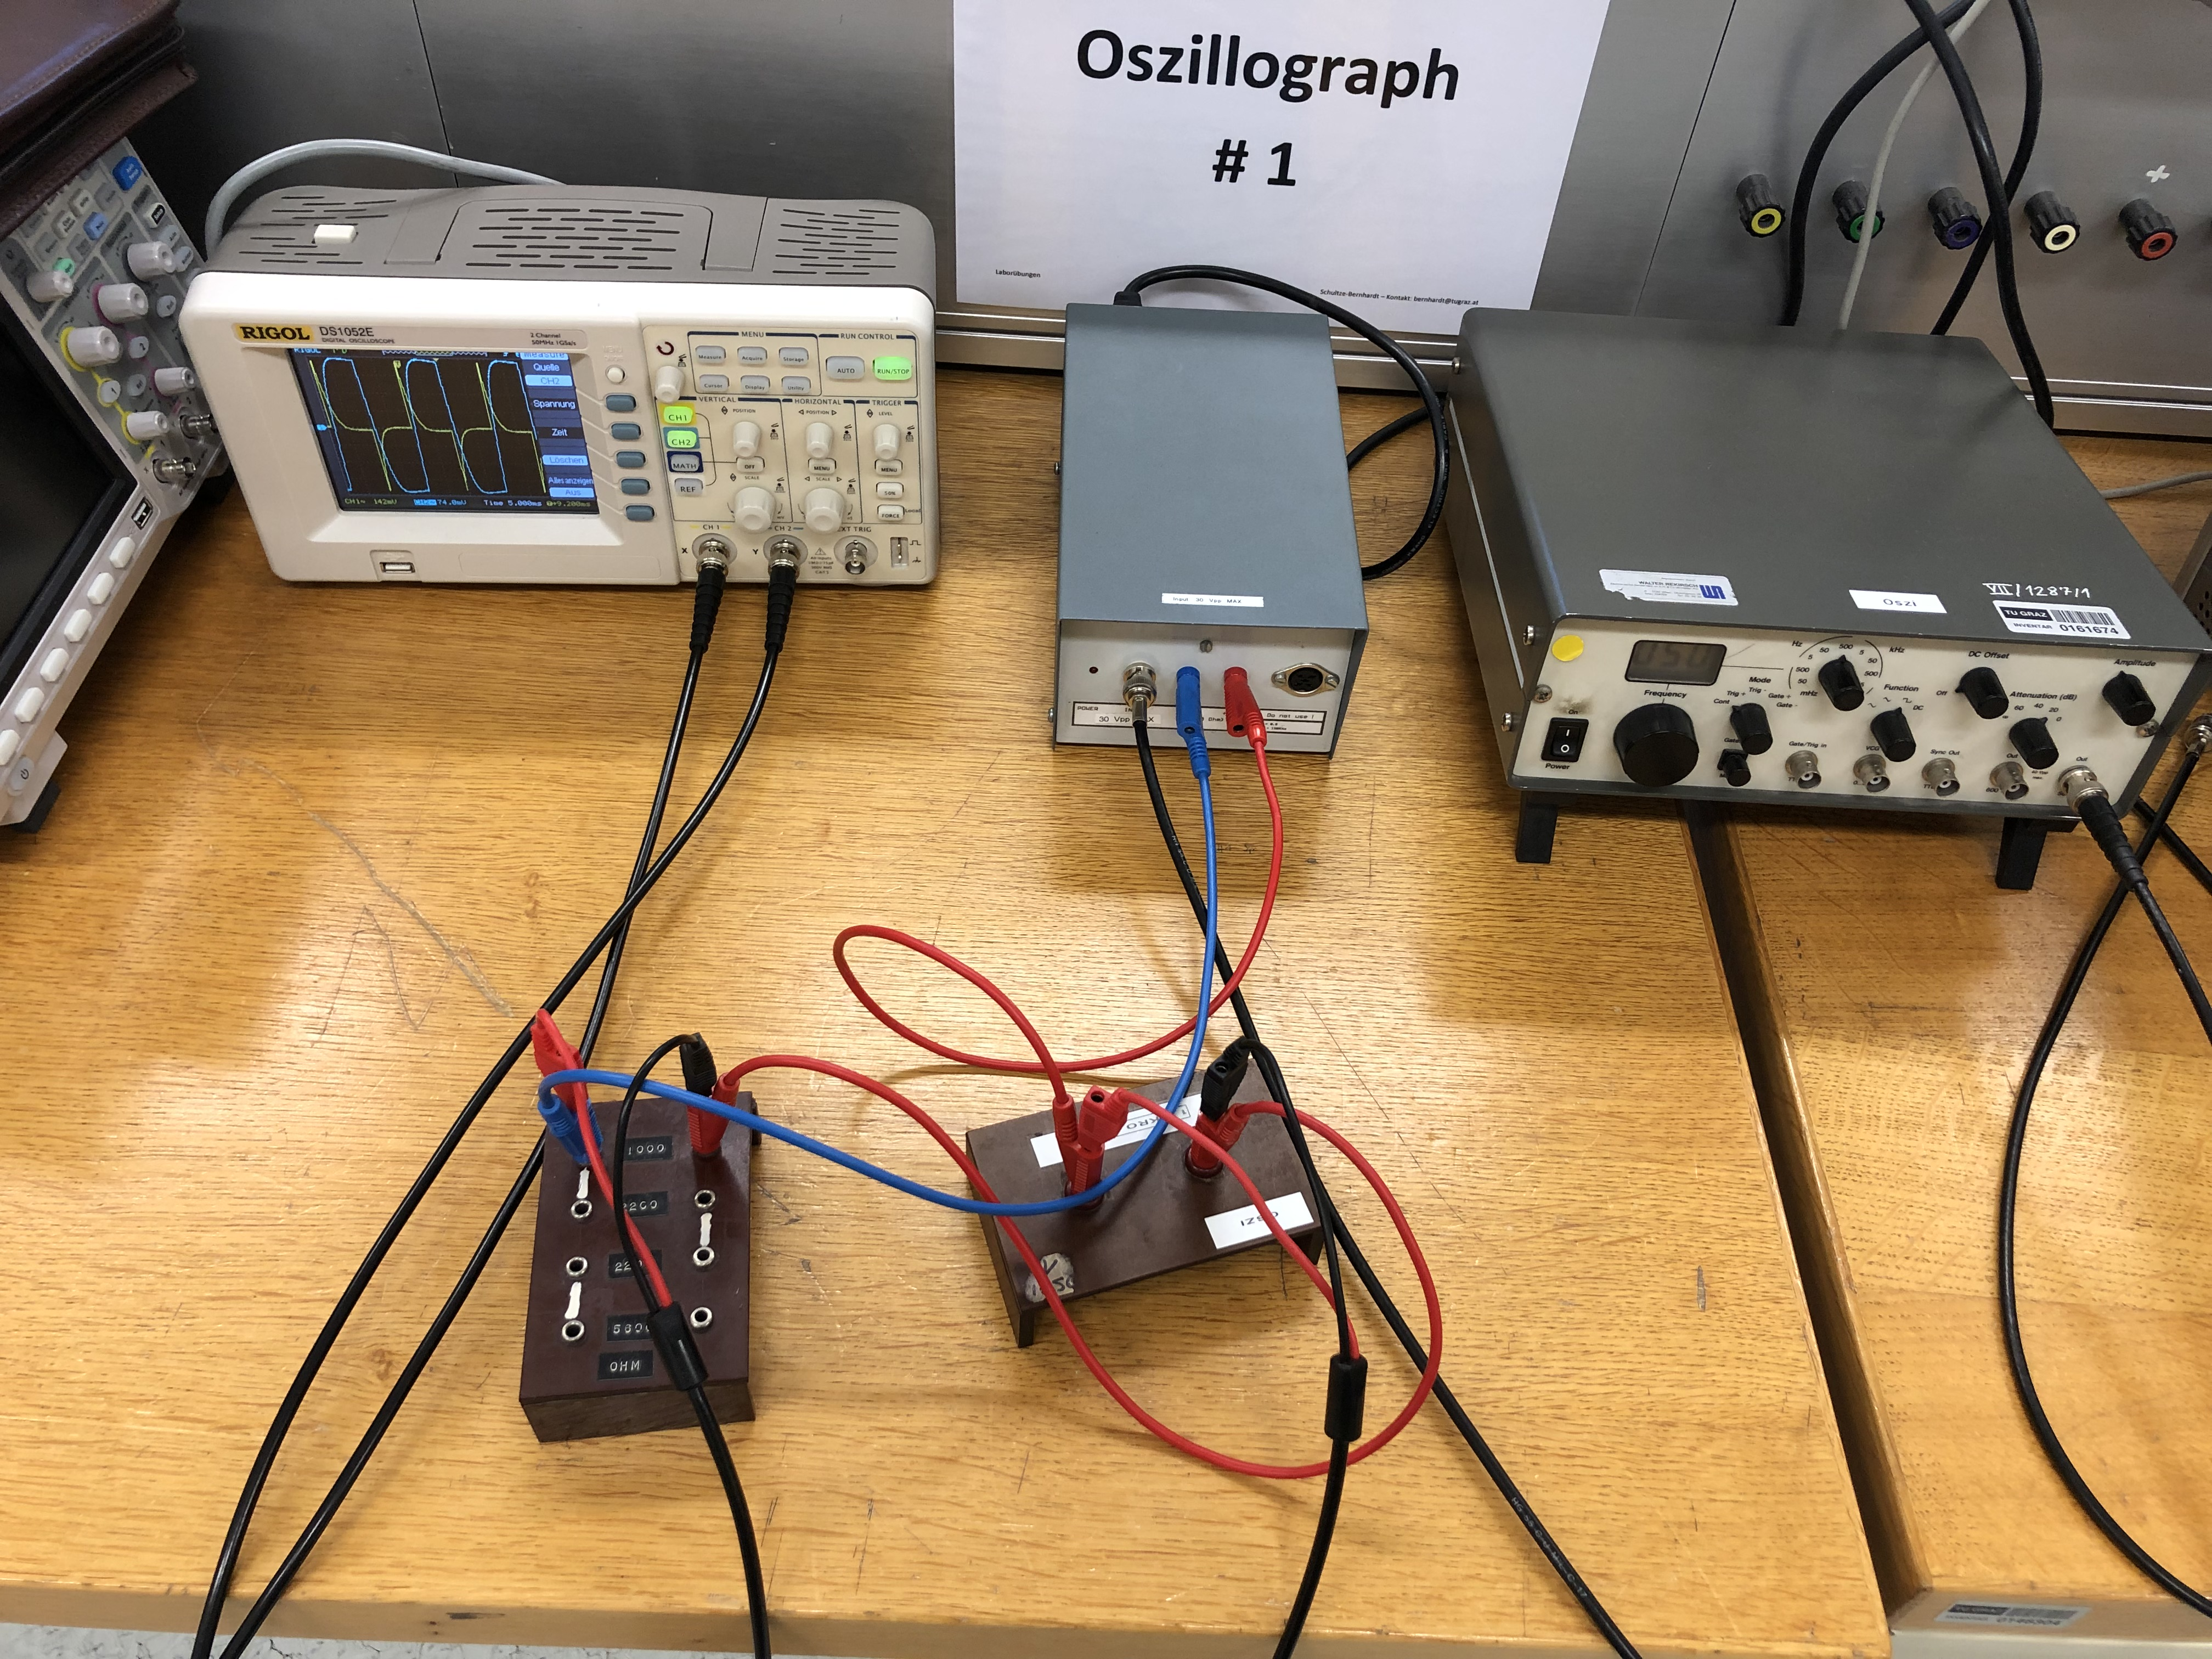
\includegraphics[width=0.7\textwidth]{aufbau_c}
	\end{center}
	\caption{Versuchsaufbau für die Serienschaltung aus ohm´schen Widerstand und Kapazität}
	\label{fig:aufbau_c}
\end{figure}

Für diesen Teil des Versuchs wird ein Widerstand von \SI{1000(100)}{\ohm}, sowie ein Kondensator mit einer Kapazität von \SI{1.00(10)}{\micro\farad}	 verwendet. Das Ausgangssignal des Generators beträgt \SI{50(1)}{\hertz}. Beim Oszilloskop ist zu beachten, dass das Signal auf CH1 noch invertiert werden muss, um sicherzustellen, dass die Phasenverschiebung richtig dargestellt wird. Zunächst wird eine Sinusspannung angelegt, wodurch folgende Grafik am Oszilloskop entsteht.

\begin{figure}[H]
	\begin{center}
		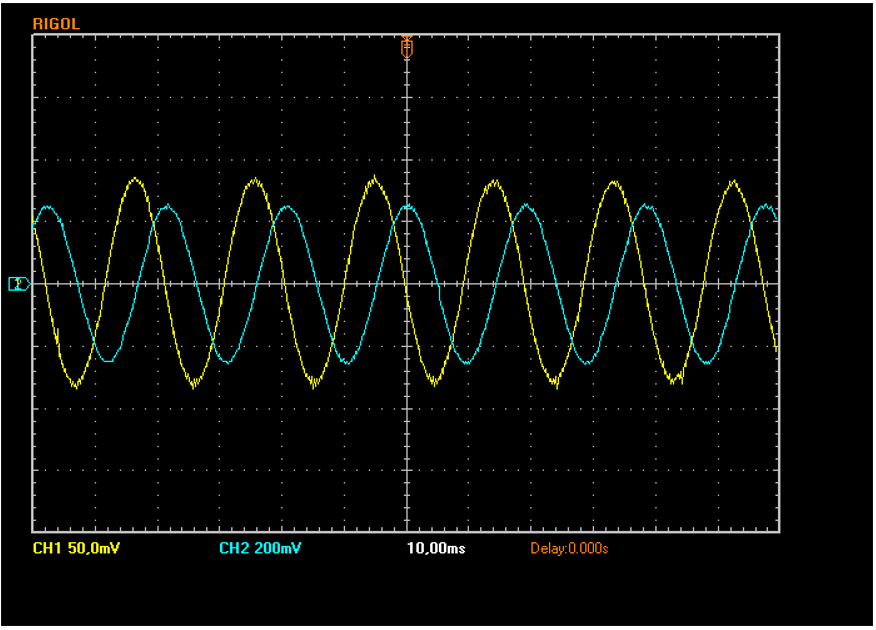
\includegraphics[width=0.7\textwidth]{Bild_versuch1}
	\end{center}
	\caption{Aufgezeichnetes Signal am Oszilloskop bei einer Sinusspannung mit einer Frequenz von \SI{50(1)}{\hertz}}
	\label{fig:sinusschw}
\end{figure}

Dabei ist zu beachten, dass es sich bei beiden Kurven um Spannungen handelt, die um den Faktor 1000 proportional zum Strom skaliert sind.

Die so erhaltene Grafik wird mithilfe des Computerprogramms ``Ultrascope`` ausgewertet und die erhaltenen Daten als ``xls-Datei`` abgespeichert.

\vspace{2mm}

Nun wird eine Rechteckspannung mit einer Frequenz von \SI{50(1)}{\hertz} angelegt, wodurch sich folgende Grafik ergibt.

\begin{figure}[H]
	\begin{center}
		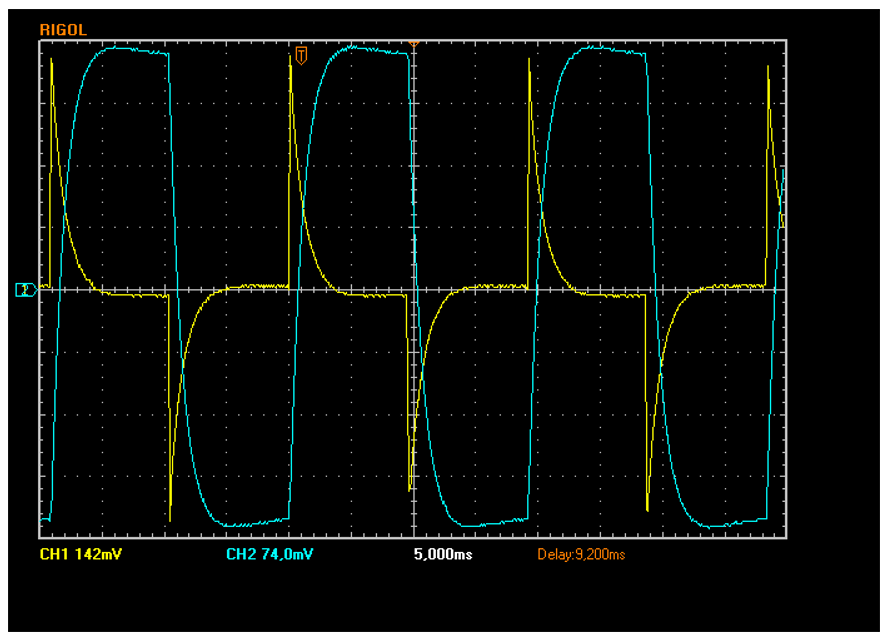
\includegraphics[width=0.7\textwidth]{Bild_versuch2}
	\end{center}
	\caption{Aufgezeichnetes Signal am Oszilloskop bei einer Rechteckspannung mit einer Frequenz von \SI{50(1)}{\hertz}}
	\label{fig:rechteckschw}
\end{figure}

Um nun die Abklingzeit der Rechteckspannung zu bestimmen wird das zuvor bestimmte Signal am Oszilloskop vergrößert, sodass nur noch eine Periode sichtbar wird, wodurch folgende Grafik entsteht.

\begin{figure}[H]
	\begin{center}
		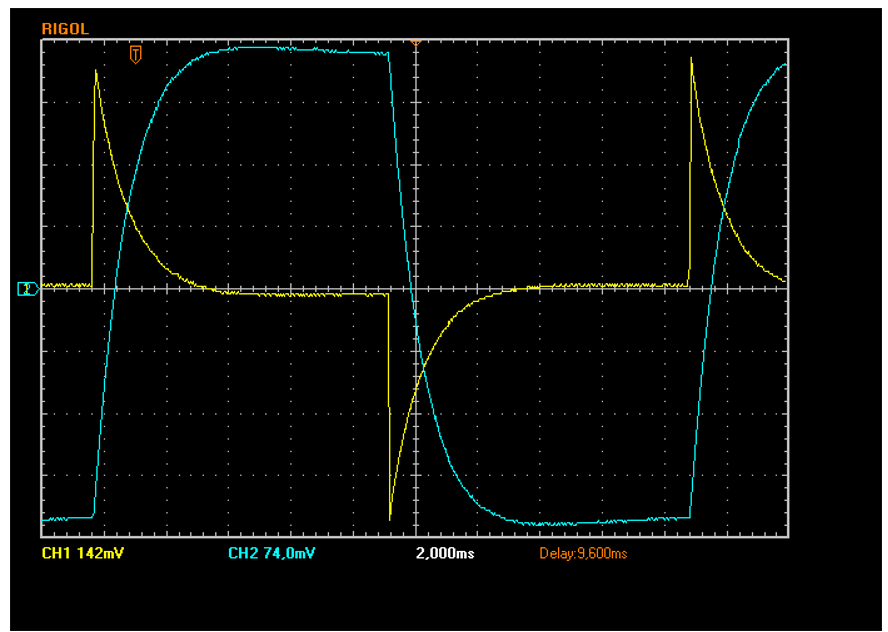
\includegraphics[width=0.7\textwidth]{Bild_versuch2_b}
	\end{center}
	\caption{Vergrößerter Ausschnitt des aufgezeichneten Signal am Oszilloskop bei einer Rechteckspannung mit einer Frequenz von \SI{50(1)}{\hertz}}
	\label{fig:rechteckschw_groß}
\end{figure}

Auch diese Grafik und Daten werden mithilfe des Computerprogramms ``Ultrascope`` gespeichert. Weil die so erhaltenen Daten nur als
``xls-Datei``
gespeichert wurden und so nicht weiterverwendet werden können, werden diese nochmals separat direkt am Oszilloskop als ``CSV-Datei`` abgespeichert.


\subsection{Serienschwingkreis}

Für diesen Teil des Versuchs wurde der Stromkreis nach der Skizze in \autoref{fig:abb6} aufgebaut, wodurch sich folgender Aufbau ergibt. Das Oszilloskop wird dabei über den Widerstand in den Stromkreis angeschlossen.

\begin{figure}[H]
	\begin{center}
		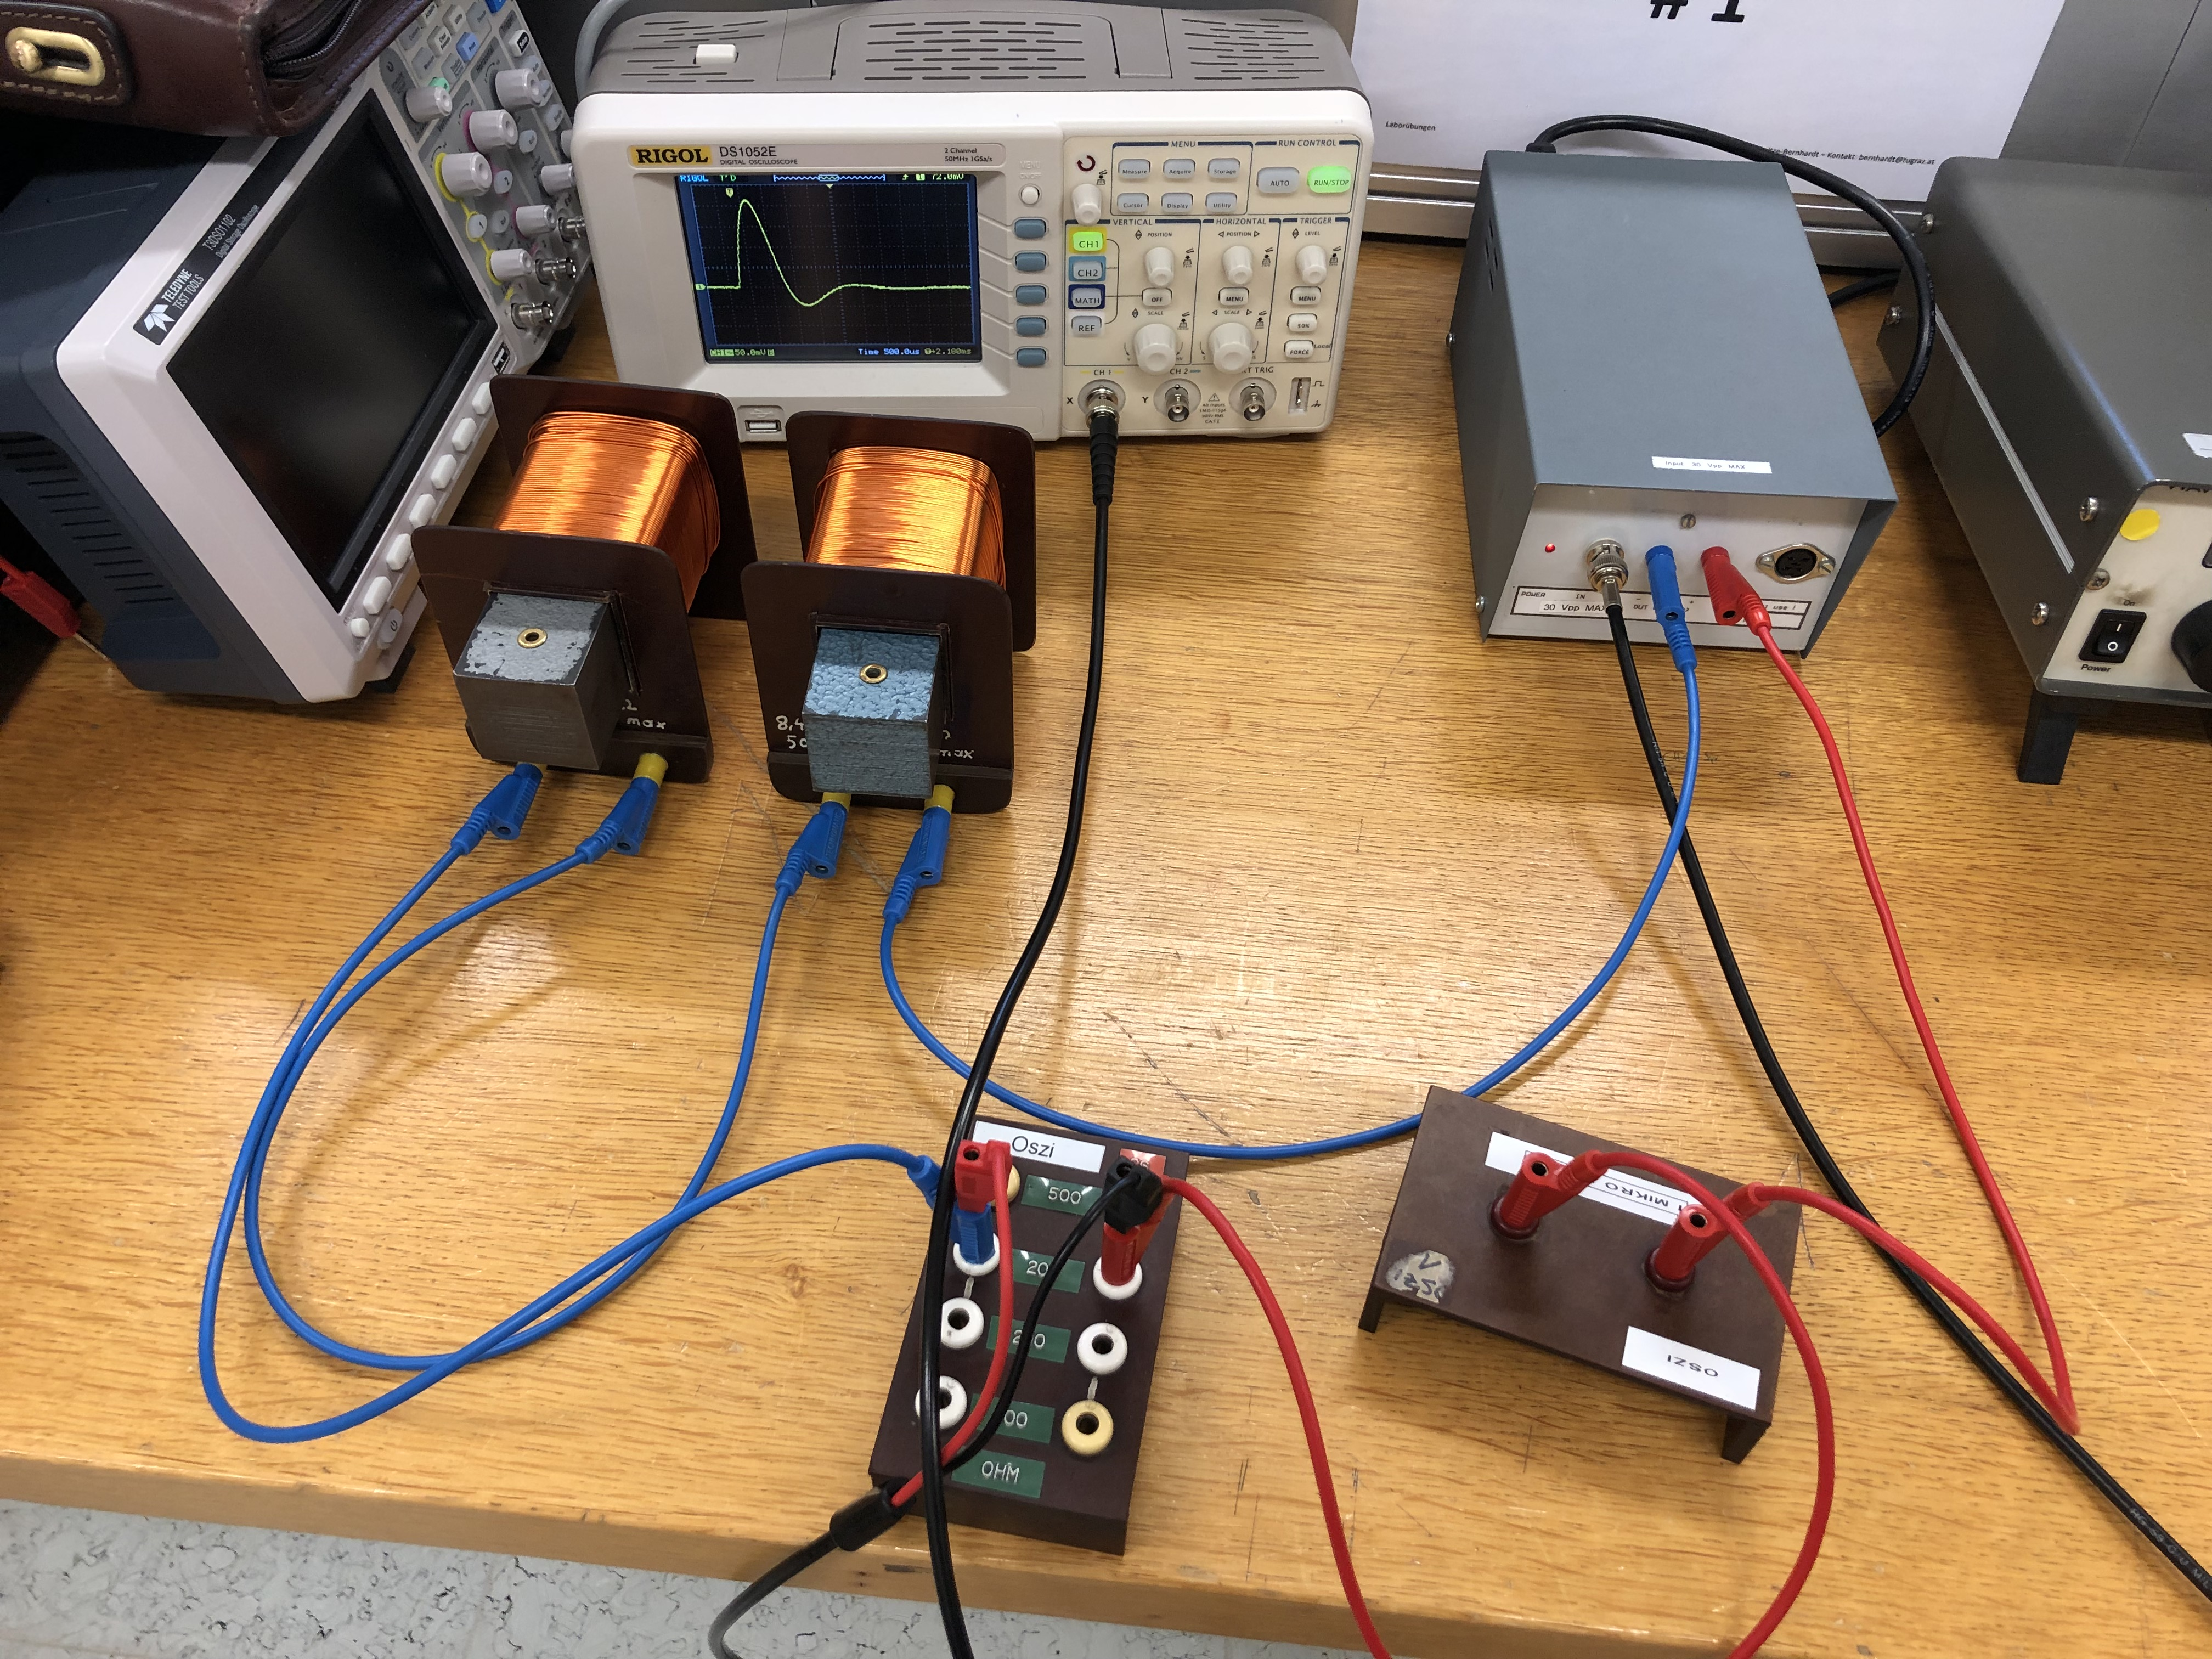
\includegraphics[width=0.7\textwidth]{aufbau_spule}
	\end{center}
	\caption{Versuchsaufbau für den Serienschwingkreis}
	\label{fig:aufbau_spule}
\end{figure}

Um die einzelnen Schwingfälle zu ermöglichen, werden in die Spulen der Reihe nach Eisenkerne eingeschoben.

Ohne die Eisenkerne ergibt sich folgende Grafik, die den Kriechfall darstellt.

\begin{figure}[H]
	\begin{center}
		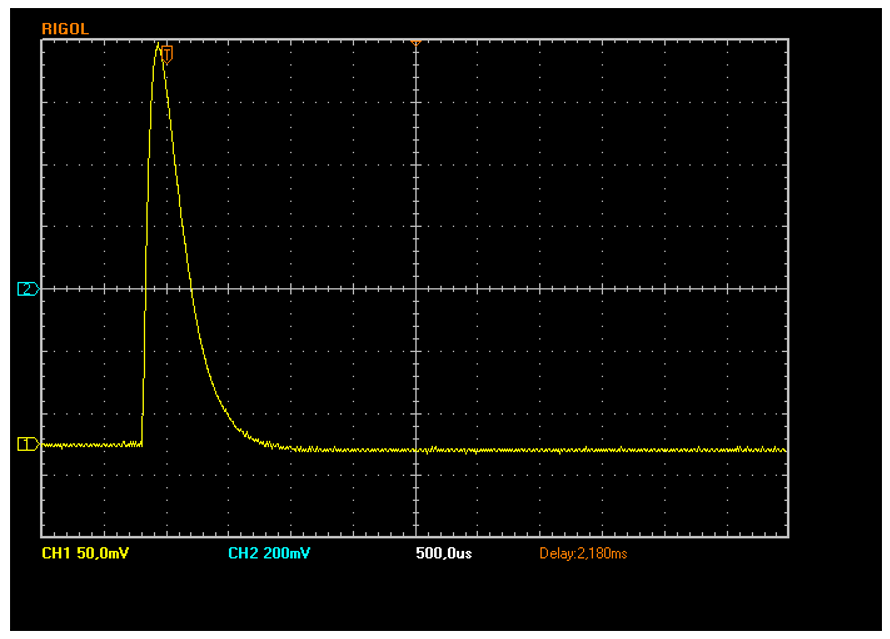
\includegraphics[width=0.7\textwidth]{Bild_versuch3_a}
	\end{center}
	\caption{Aufgezeichnetes Signal des Kriechfalls}
	\label{fig:kriechfall}
\end{figure}

Nun wird ein Eisenkern so weit in die erste Spule eingeschoben, wie in \autoref{fig:einschub}ersichtlich, bis die Kurve kurz vor dem Durchschwingen ist, was den aperiodischen Grenzfall darstellt, wie in folgender Grafik ersichtlich.

\begin{figure}[H]
	\begin{center}
		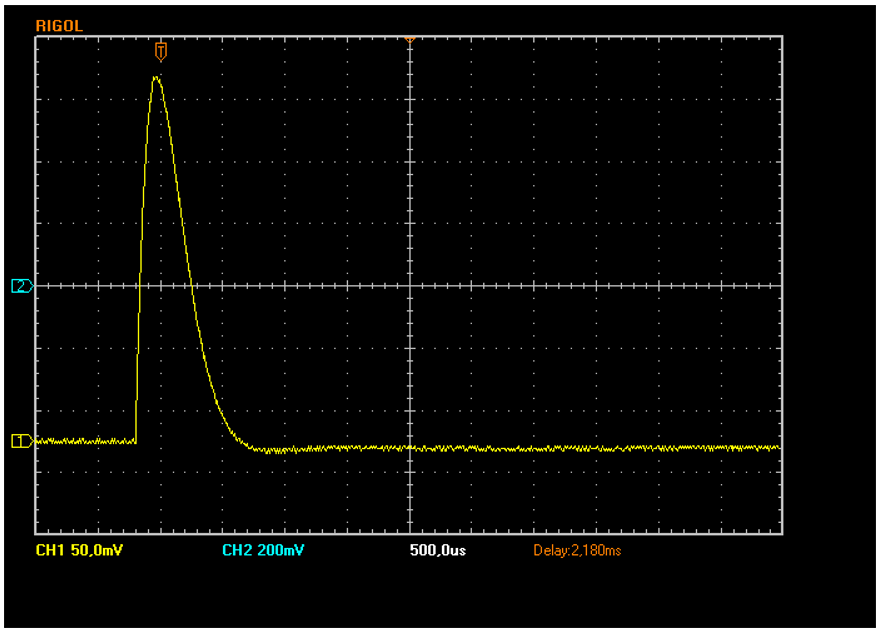
\includegraphics[width=0.7\textwidth]{Bild_versuch3_b}
	\end{center}
	\caption{Aufgezeichnetes Signal des Grenzfalls}
	\label{fig:grenzfall}
\end{figure}

\begin{figure}[H]
	\begin{center}
		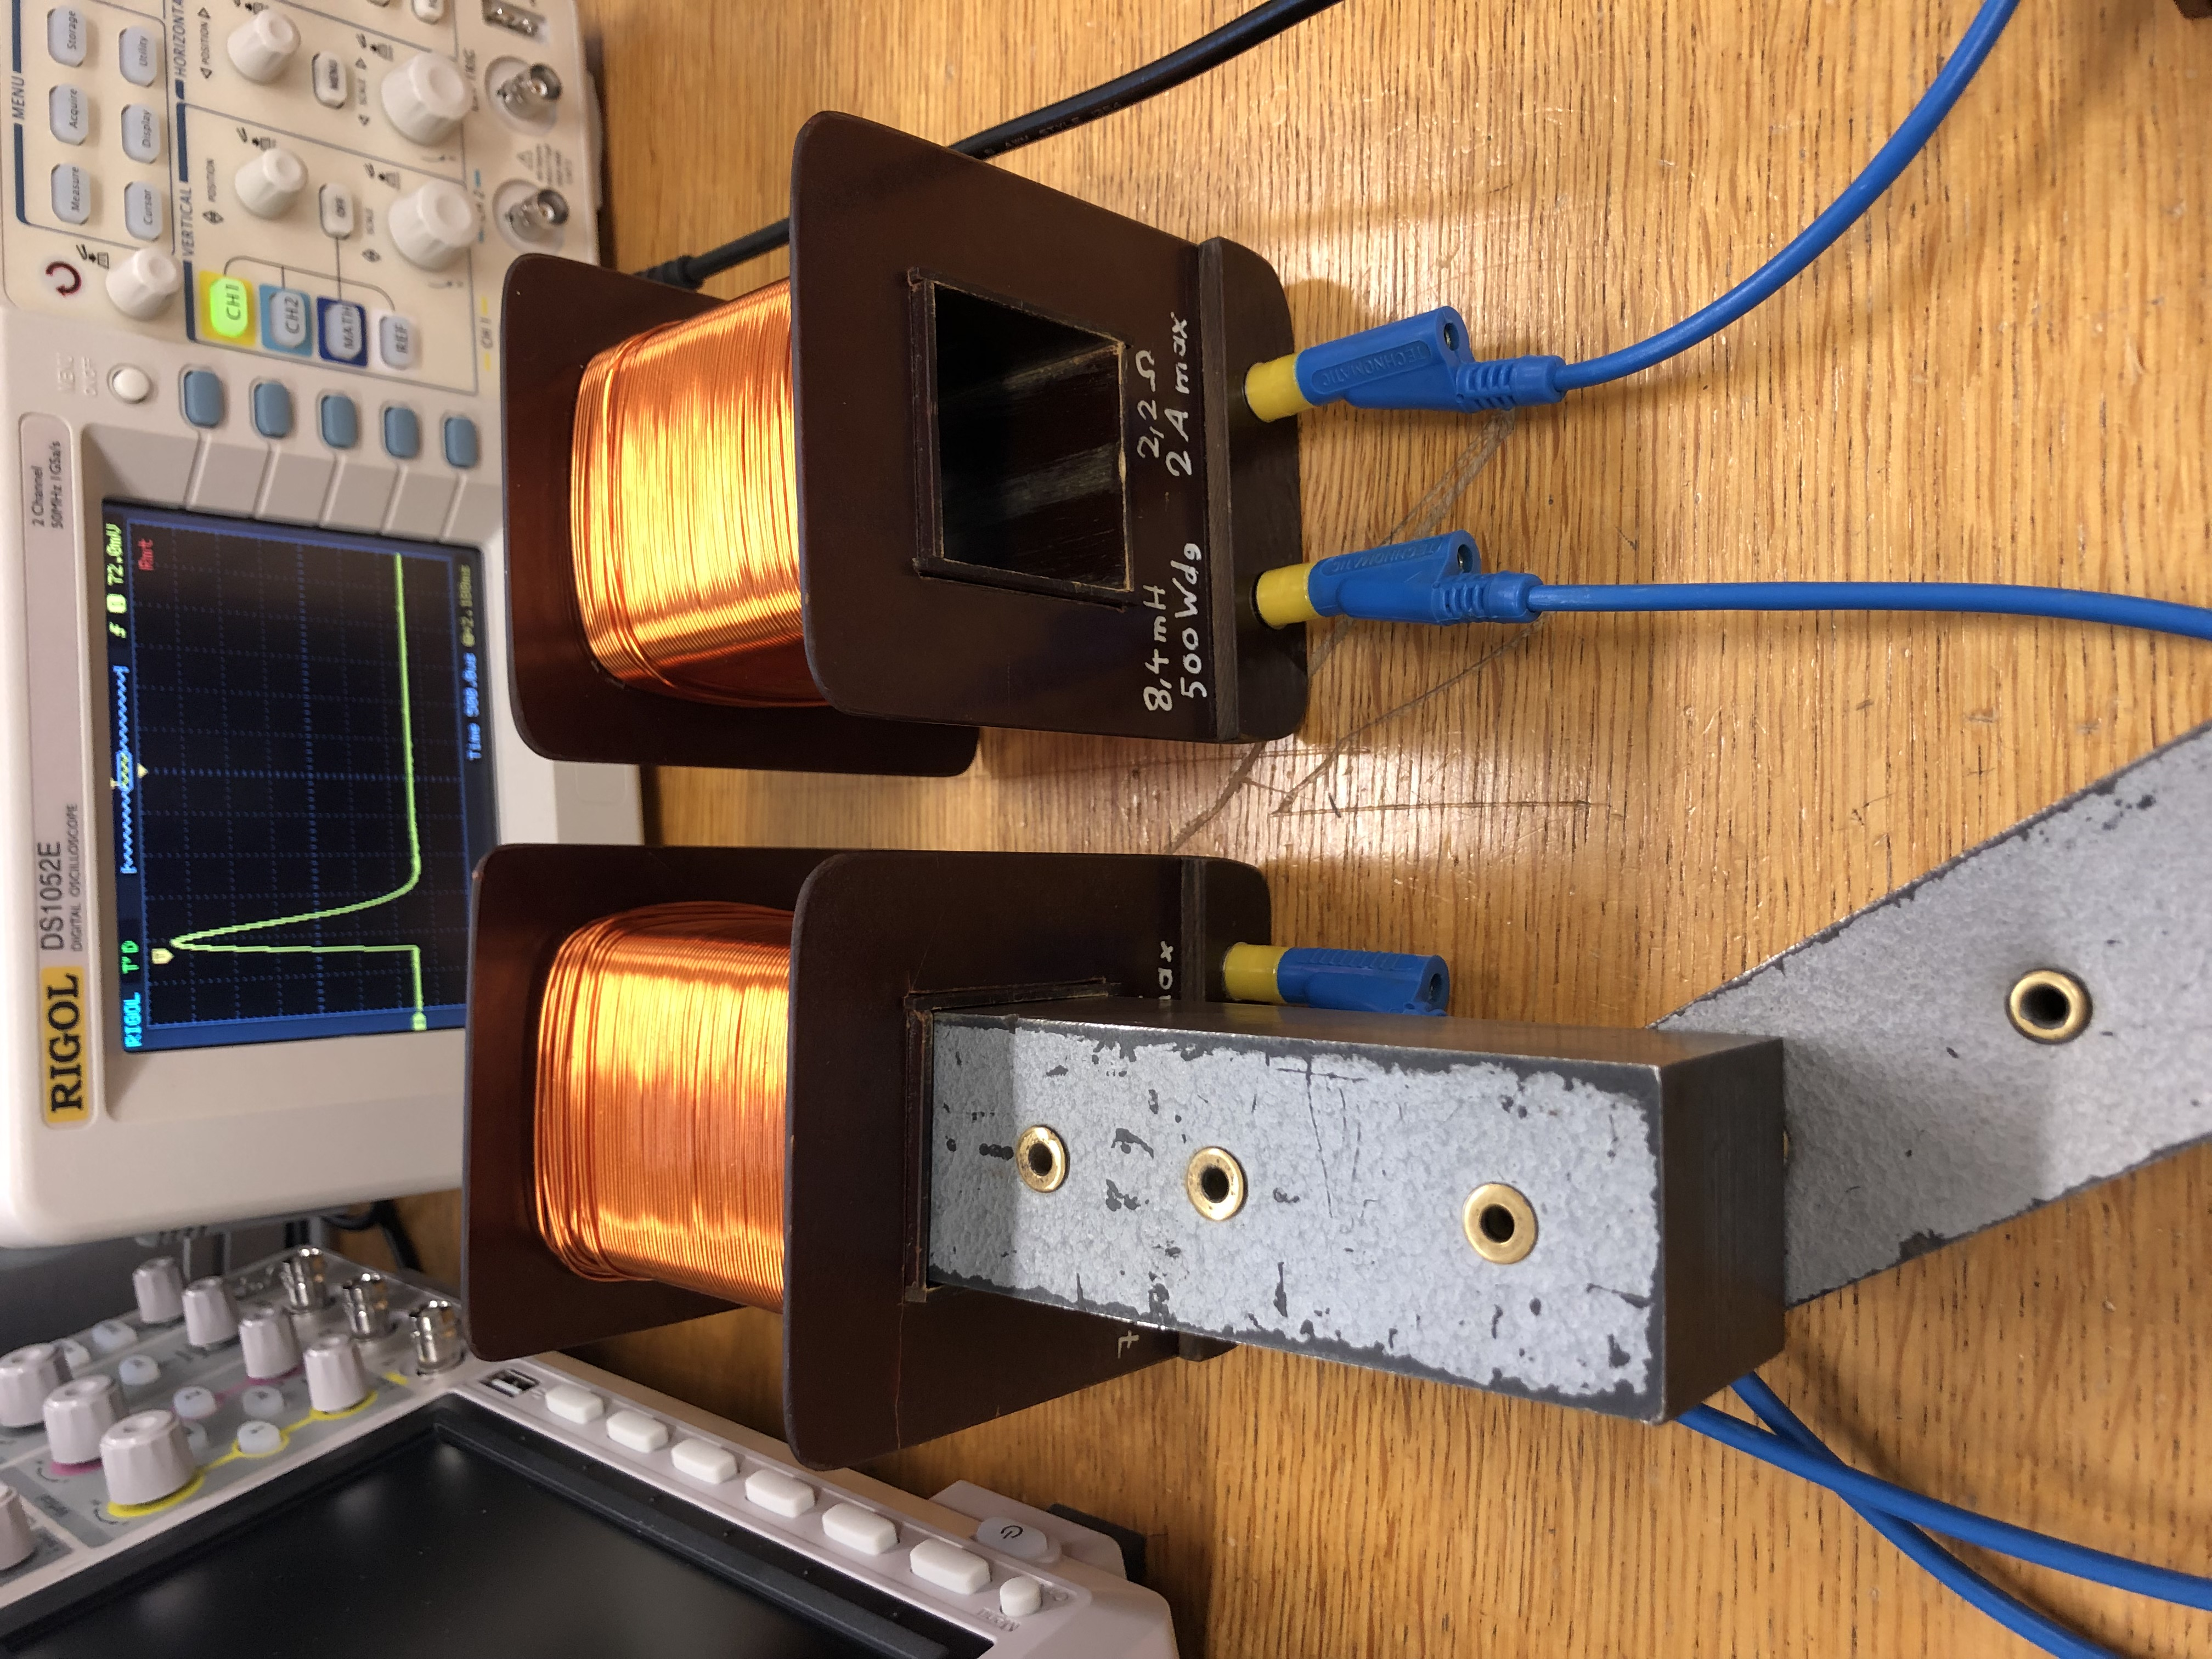
\includegraphics[angle=-90,width=0.5\textwidth]{einschub}
	\end{center}
	\caption{Eingeschobener Eisenkern für den Kriechfall}
	\label{fig:einschub}
\end{figure}

Zuletzt werden beide Einsenkerne noch in die Spulen eingeschoben, was den Schwingfall des Serienschwingkreises repräsentiert, wie in folgender Grafik sichtbar.

\begin{figure}[H]
	\begin{center}
		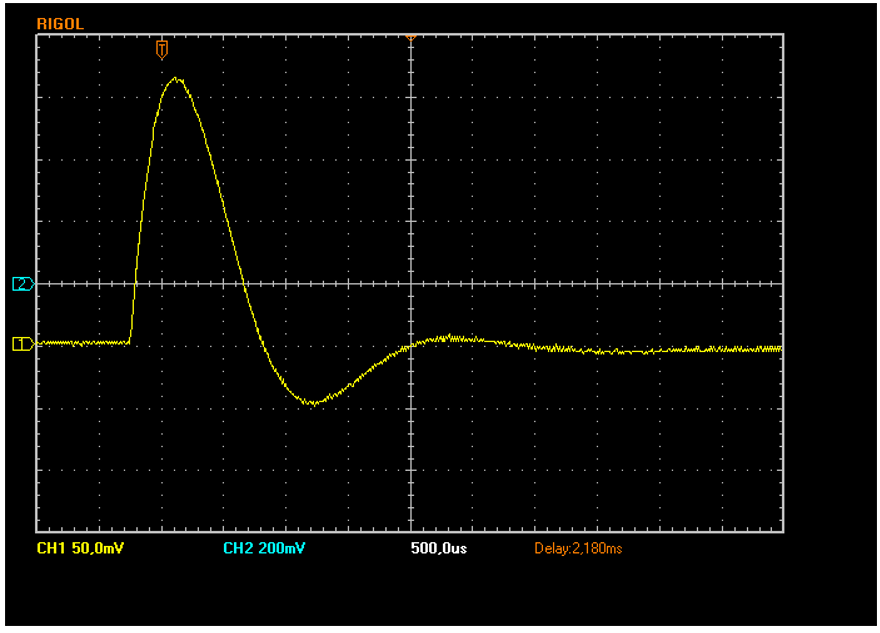
\includegraphics[width=0.7\textwidth]{Bild_versuch3_c}
	\end{center}
	\caption{Aufgezeichnetes Signal des Schwingfalls}
	\label{fig:schwingfall}
\end{figure}


\section{Auswertung}

\noindent Um zu sehen wie sich die Unsicherheit der Messungen bis in die Ergebnisse
fortplanzt, ist \autoref{eq:Unsicherheitsfortpflanzung} verwendet worden.
Die Grundlagen dieser Gleichung stammen von den Powerpointfolien von
GUM.\cite{WolfgangKessel2004} Die Verallgemeinerung ist von Wikipedia entnommen
worden \cite{2020Fehler}.
Für die Auswertung ist die Progammiersprache Python im speziellen das
Packet \verb#scipy#, zur Hilfe genommen worden.

\begin{equation}
	\label{eq:Unsicherheitsfortpflanzung}
	V_y = J(x) \cdot V_x \cdot J^{T}(x)
\end{equation}

\noindent Wobei $V_y$ und $V_x$ die Kovarianzmatrizen von den Vektoren $\bm{y}$ und $\bm{x}$ sind.
$\bm{x}$ ist der Vektor der Eingangsvariablen und $\bm{y}$ ist der Vektor der Ausgangsvariablen.
$J$ ist die Jakobimatrix der vektorwertigen Funktion $\bm{y} = \vec{F}(\bm{x})$.
So lassen sich die Komponenten der Matrix relativ einfach anschreiben $J_{ij}(x) = \frac{\partial{y_i}}{\partial{x_j}}(x)$.
Damit man die Unsicherheit der einzelnen Variablen $y_i$ bekommt, muss nur die Quadratwurzel des i-ten Diagonalelementes der
$\bm{y}$-Kovarianzmatrix genommen werden $u_i= \sqrt{\mathrm{diag}(V_y)_i}$.
Da in diesem Experiment meistens nur skalare Funktionen untersucht werden, vereinfacht
sich die \autoref{eq:Unsicherheitsfortpflanzung} dramatisch und die Unsicherheit
der Variable $y$ lässt sich einfach so berechnen:

\begin{equation}
	\label{eq:graduncentainty}
	u_y = \sqrt{\mathrm{grad} y^T \cdot V_x \cdot \mathrm{grad} y}
\end{equation}

Für die Unsicherheit der Bauteile wurde dabei ein Wert von 10 \% angenommen.

\subsection{Serienschaltung aus ohm´schen Widerstand und Kapazität}

Zunächst wurde bei der Sinusschwingung die Phasenverschiebung berechnet.
%genauer bitte !!!!!!!!!!!!!!!!!!!!!!!!!!!!!!!!!!!!!!!!!!!!!!!!!!!!!!!!!!!!!!!!

Der Strom im Schaltkreis wird nach folgender \autoref{eq:3ohm_gesetz} berechnet:

\begin{equation}
	\label{eq:3ohm_gesetz}
	I = \frac{U_R}{R}
\end{equation}

Um die Zerfallskonstante $\lambda = \frac{1}{\tau}$ zu bestimmen, wird der
entsprechende Bereich vom Entladevorgang aus den aufgezeichneten Daten
extrahiert und mit einer Exponentialfunktion gefittet, wodurch folgende Grafik
entsteht.

%fit
\begin{figure}[H]
	\begin{center}
		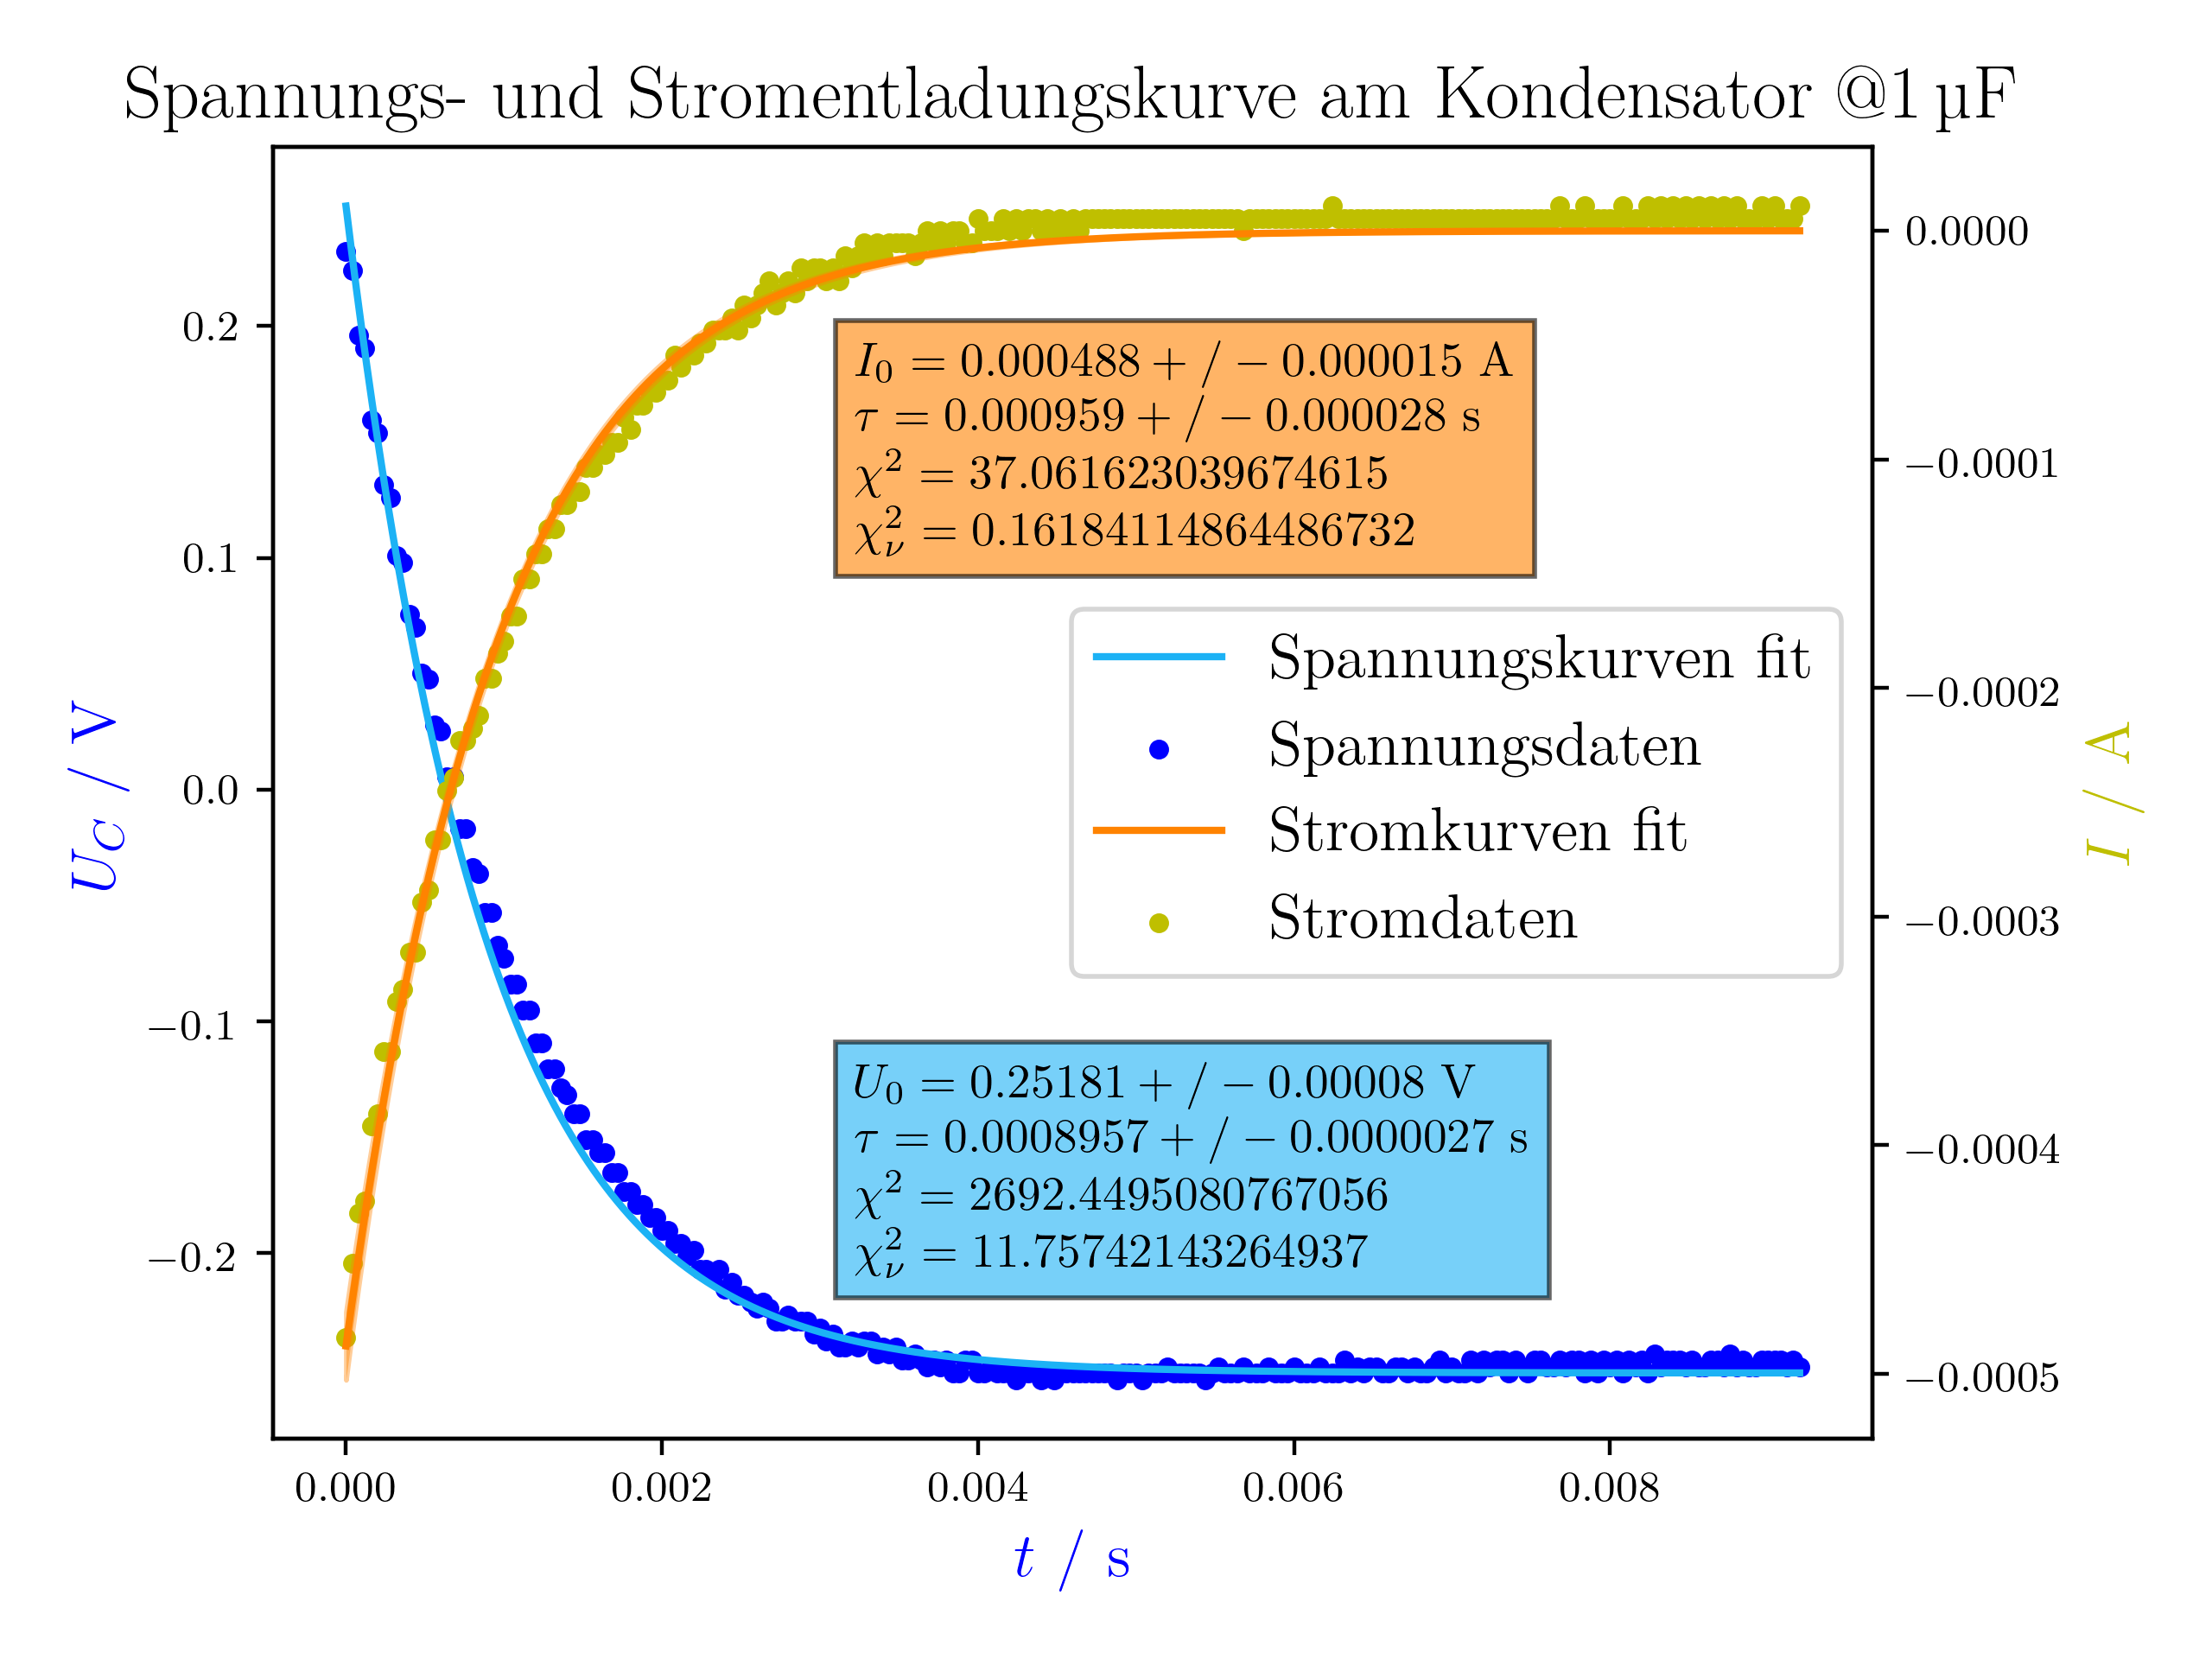
\includegraphics[width=0.95\textwidth]{figures/entladekurve}
	\end{center}
	\caption{Dies ist der Fit der Strom- (gelb) und Spannungs- (blau) Entladekurve eines RC Kreises mit einem
		Widerstand R von \SI{1000(100)}{\ohm} und einer Kapazität C von
		\SI{1.0(1)}{\micro\farad}. Die Daten sind aus \autoref{fig:rechteckschw_groß}
		entnommen worden}
	\label{fig:entladekurve}
\end{figure}

Die gefitteten Funktion sehen wie folgt aus:
\begin{align*}
	U_C & = 2U_0 e^{\frac{-t}{\tau}} - U_0 \\
	I   & = -I_0 e^{\frac{-t}{\tau}}
\end{align*}

Es wurde nicht nur der Entladevorgang aufgezeichnet, deshalb wurden zusätzlich noch die
Ladevorgänge gefittet, indem erneut der Bereich vom Ladevorgang aus aus den
aufgezeichneten Daten extrahiert und mit einer Exponentialfunktion gefittet wurde:

%fit Ladevorgang
\begin{figure}[H]
	\begin{center}
		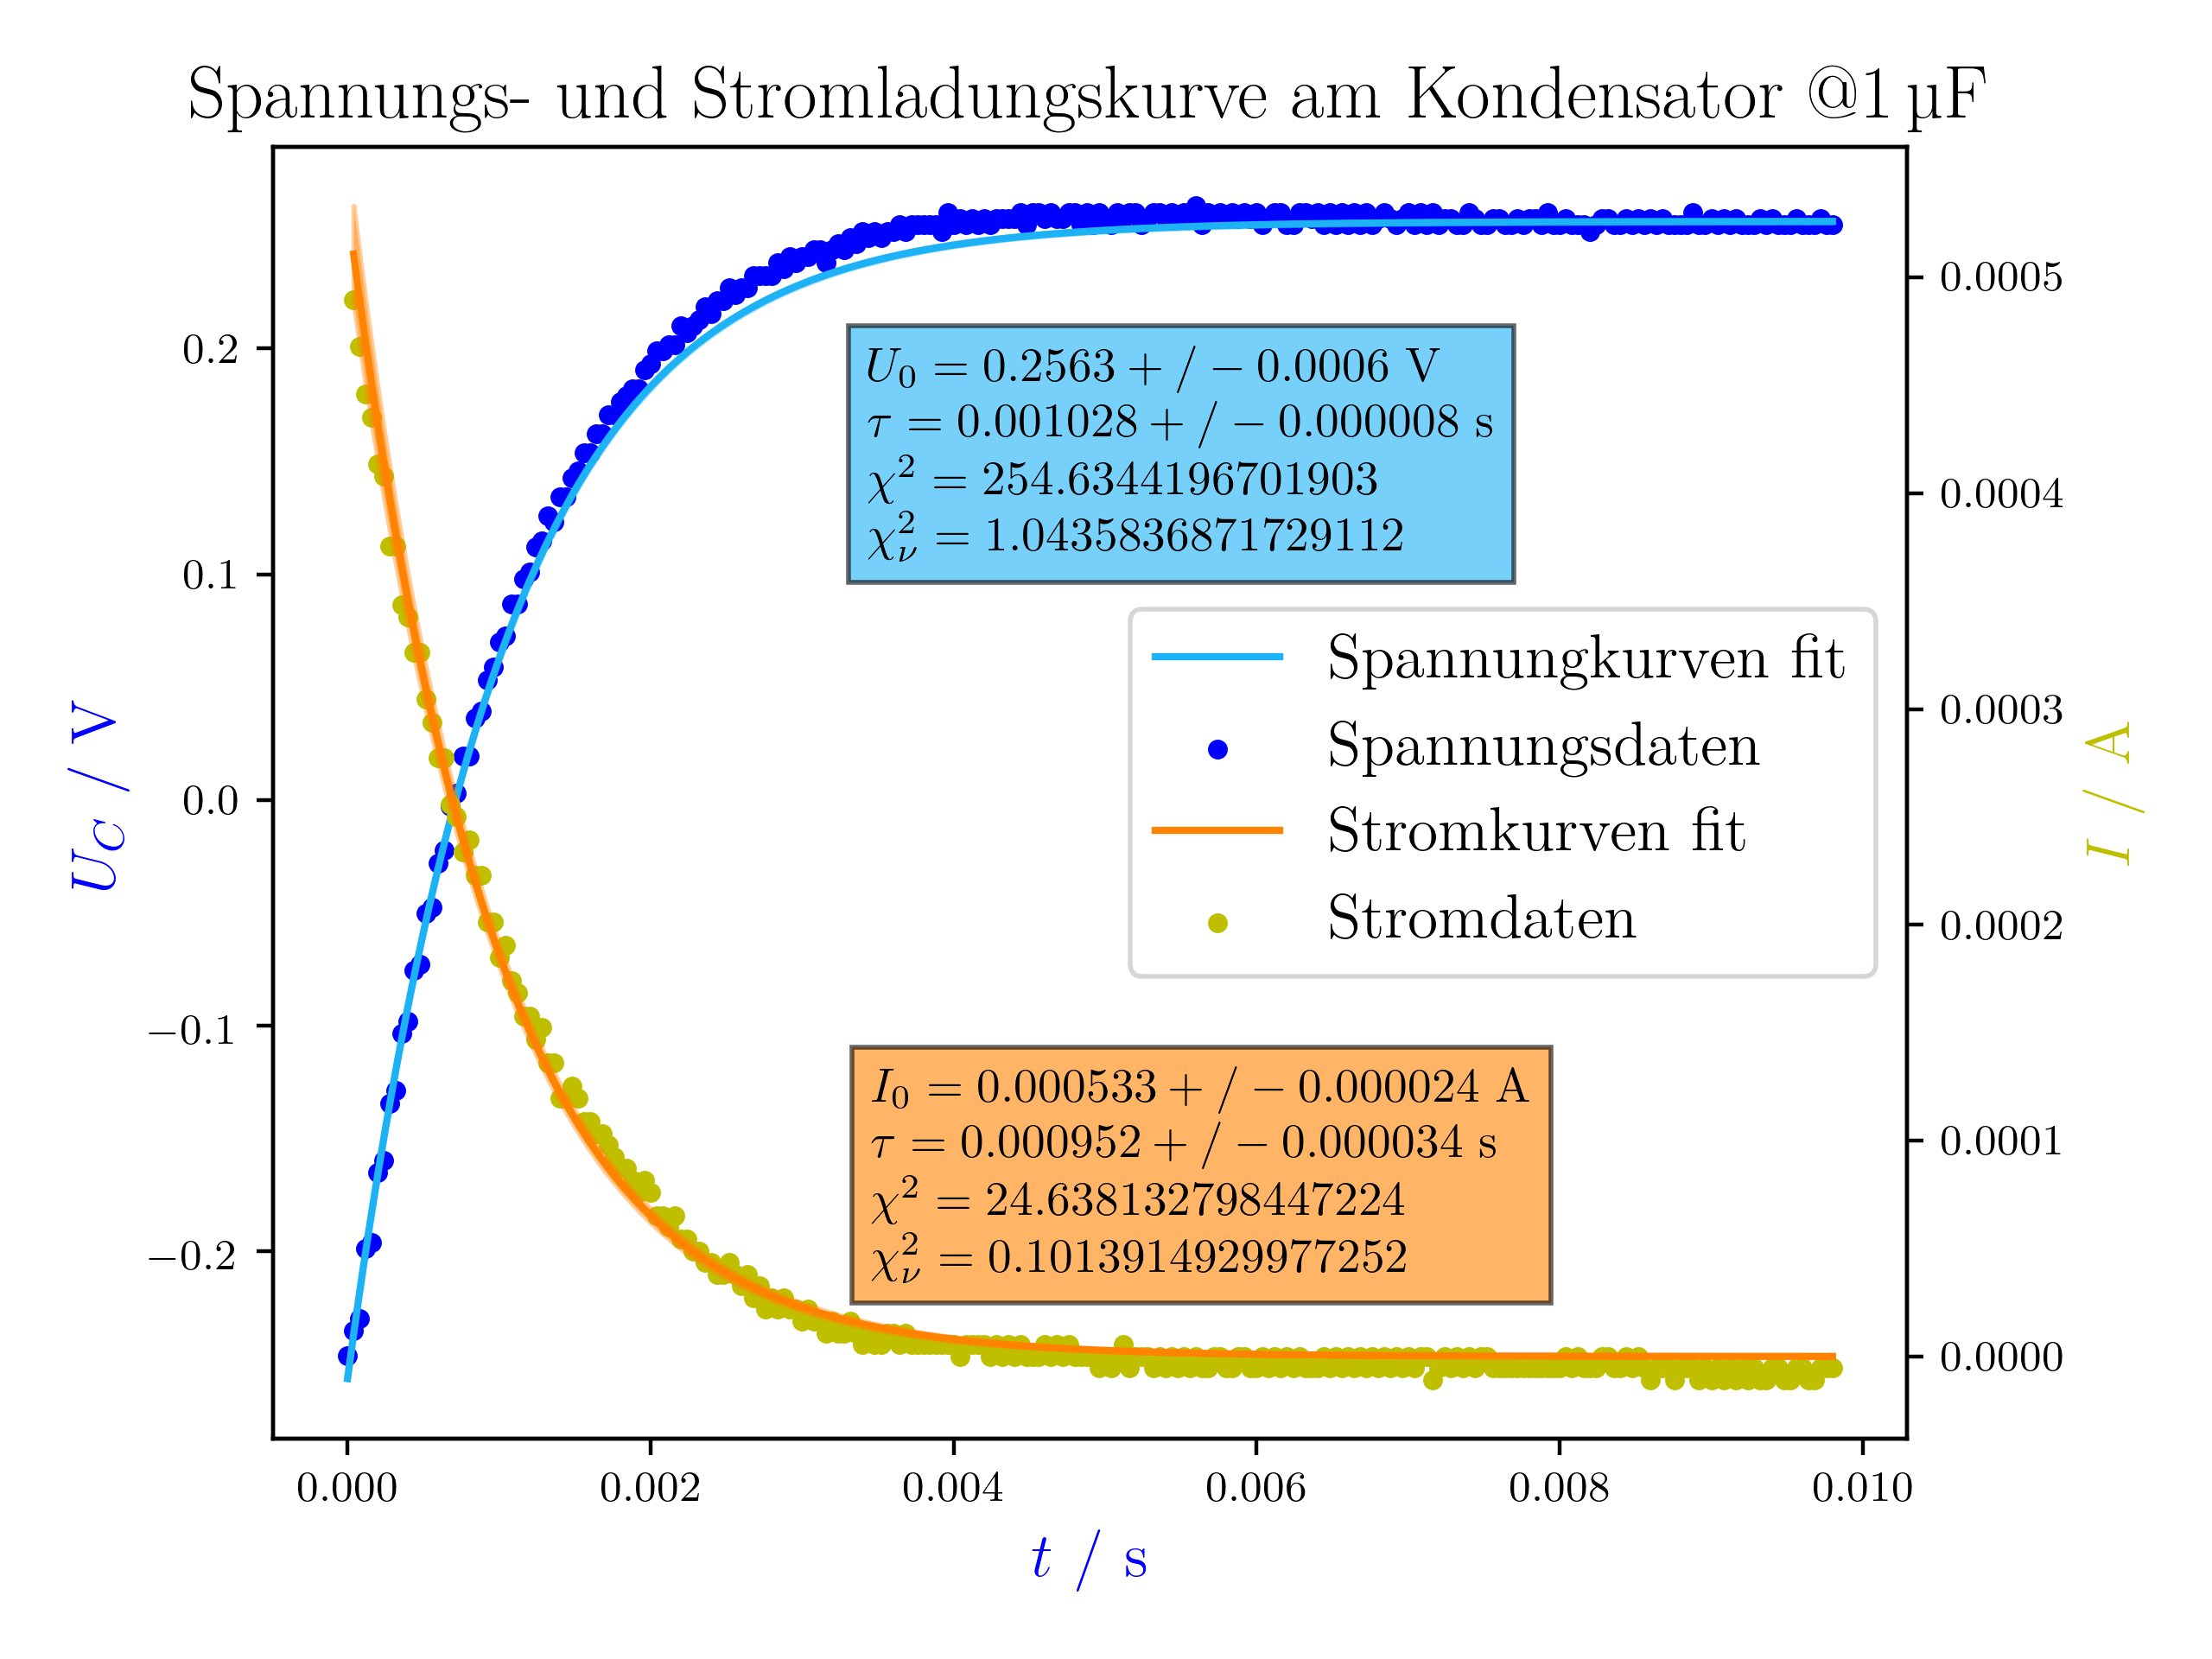
\includegraphics[width=0.95\textwidth]{figures/ladekurve}
	\end{center}
	\caption{Dies ist der Fit der Strom- (gelb) und Spannungs- (blau) Ladekurve eines RC Kreises mit einem
		Widerstand R von \SI{1000(100)}{\ohm} und einer Kapazität C von
		\SI{1.0(1)}{\micro\farad}. Die Daten sind aus \autoref{fig:rechteckschw_groß}
		entnommen worden}
	\label{fig:ladekurve}
\end{figure}

Die gefitteten Funktion haben folgende Gestalt:
\begin{align*}
	U_C & = -2U_0 e^{\frac{-t}{\tau}} + U_0 \\
	I   & = I_0 e^{\frac{-t}{\tau}}
\end{align*}

Weiters wurden auch eine Linearisierung der Daten vorgenommen indem bei den
Spannungen erst der Offset addiert wurde, damit jeder Wert größer Null
ist und Logarithmus der Daten berechnet werden kann. Das gleiche wurde auch, zur
Sicherheit, bei den Strömen gemacht, falls einen negativen Wert in den Daten auftritt.
Da das Oszilloskop nur 8 bit Auflösung hat leiden beim Logarithmus berechnen, die niedrigen
Spannungs und Stromwerte an hoher Unsicherheit und sind daher sehr verstreut. Deshalb
wurde ein Zeitabschnitt gewählt bei dem sich die Streuung der Wert noch in Grenzen hält.

Durch fitten der folgenden linearen Gleichung für die Ströme und Spannungen:

\begin{align*}
	\ln{I}   & = \frac{-t}{\tau} + \ln{I_0}  \\
	\ln{U_C} & = \frac{-t}{\tau} + \ln{2U_0}
\end{align*}

entstehen schließlich folgende Graphen:

%fit Ent & Ladevorgang Linearisierung
\begin{figure}[H]
	\centering
	\begin{minipage}{0.49\textwidth}
		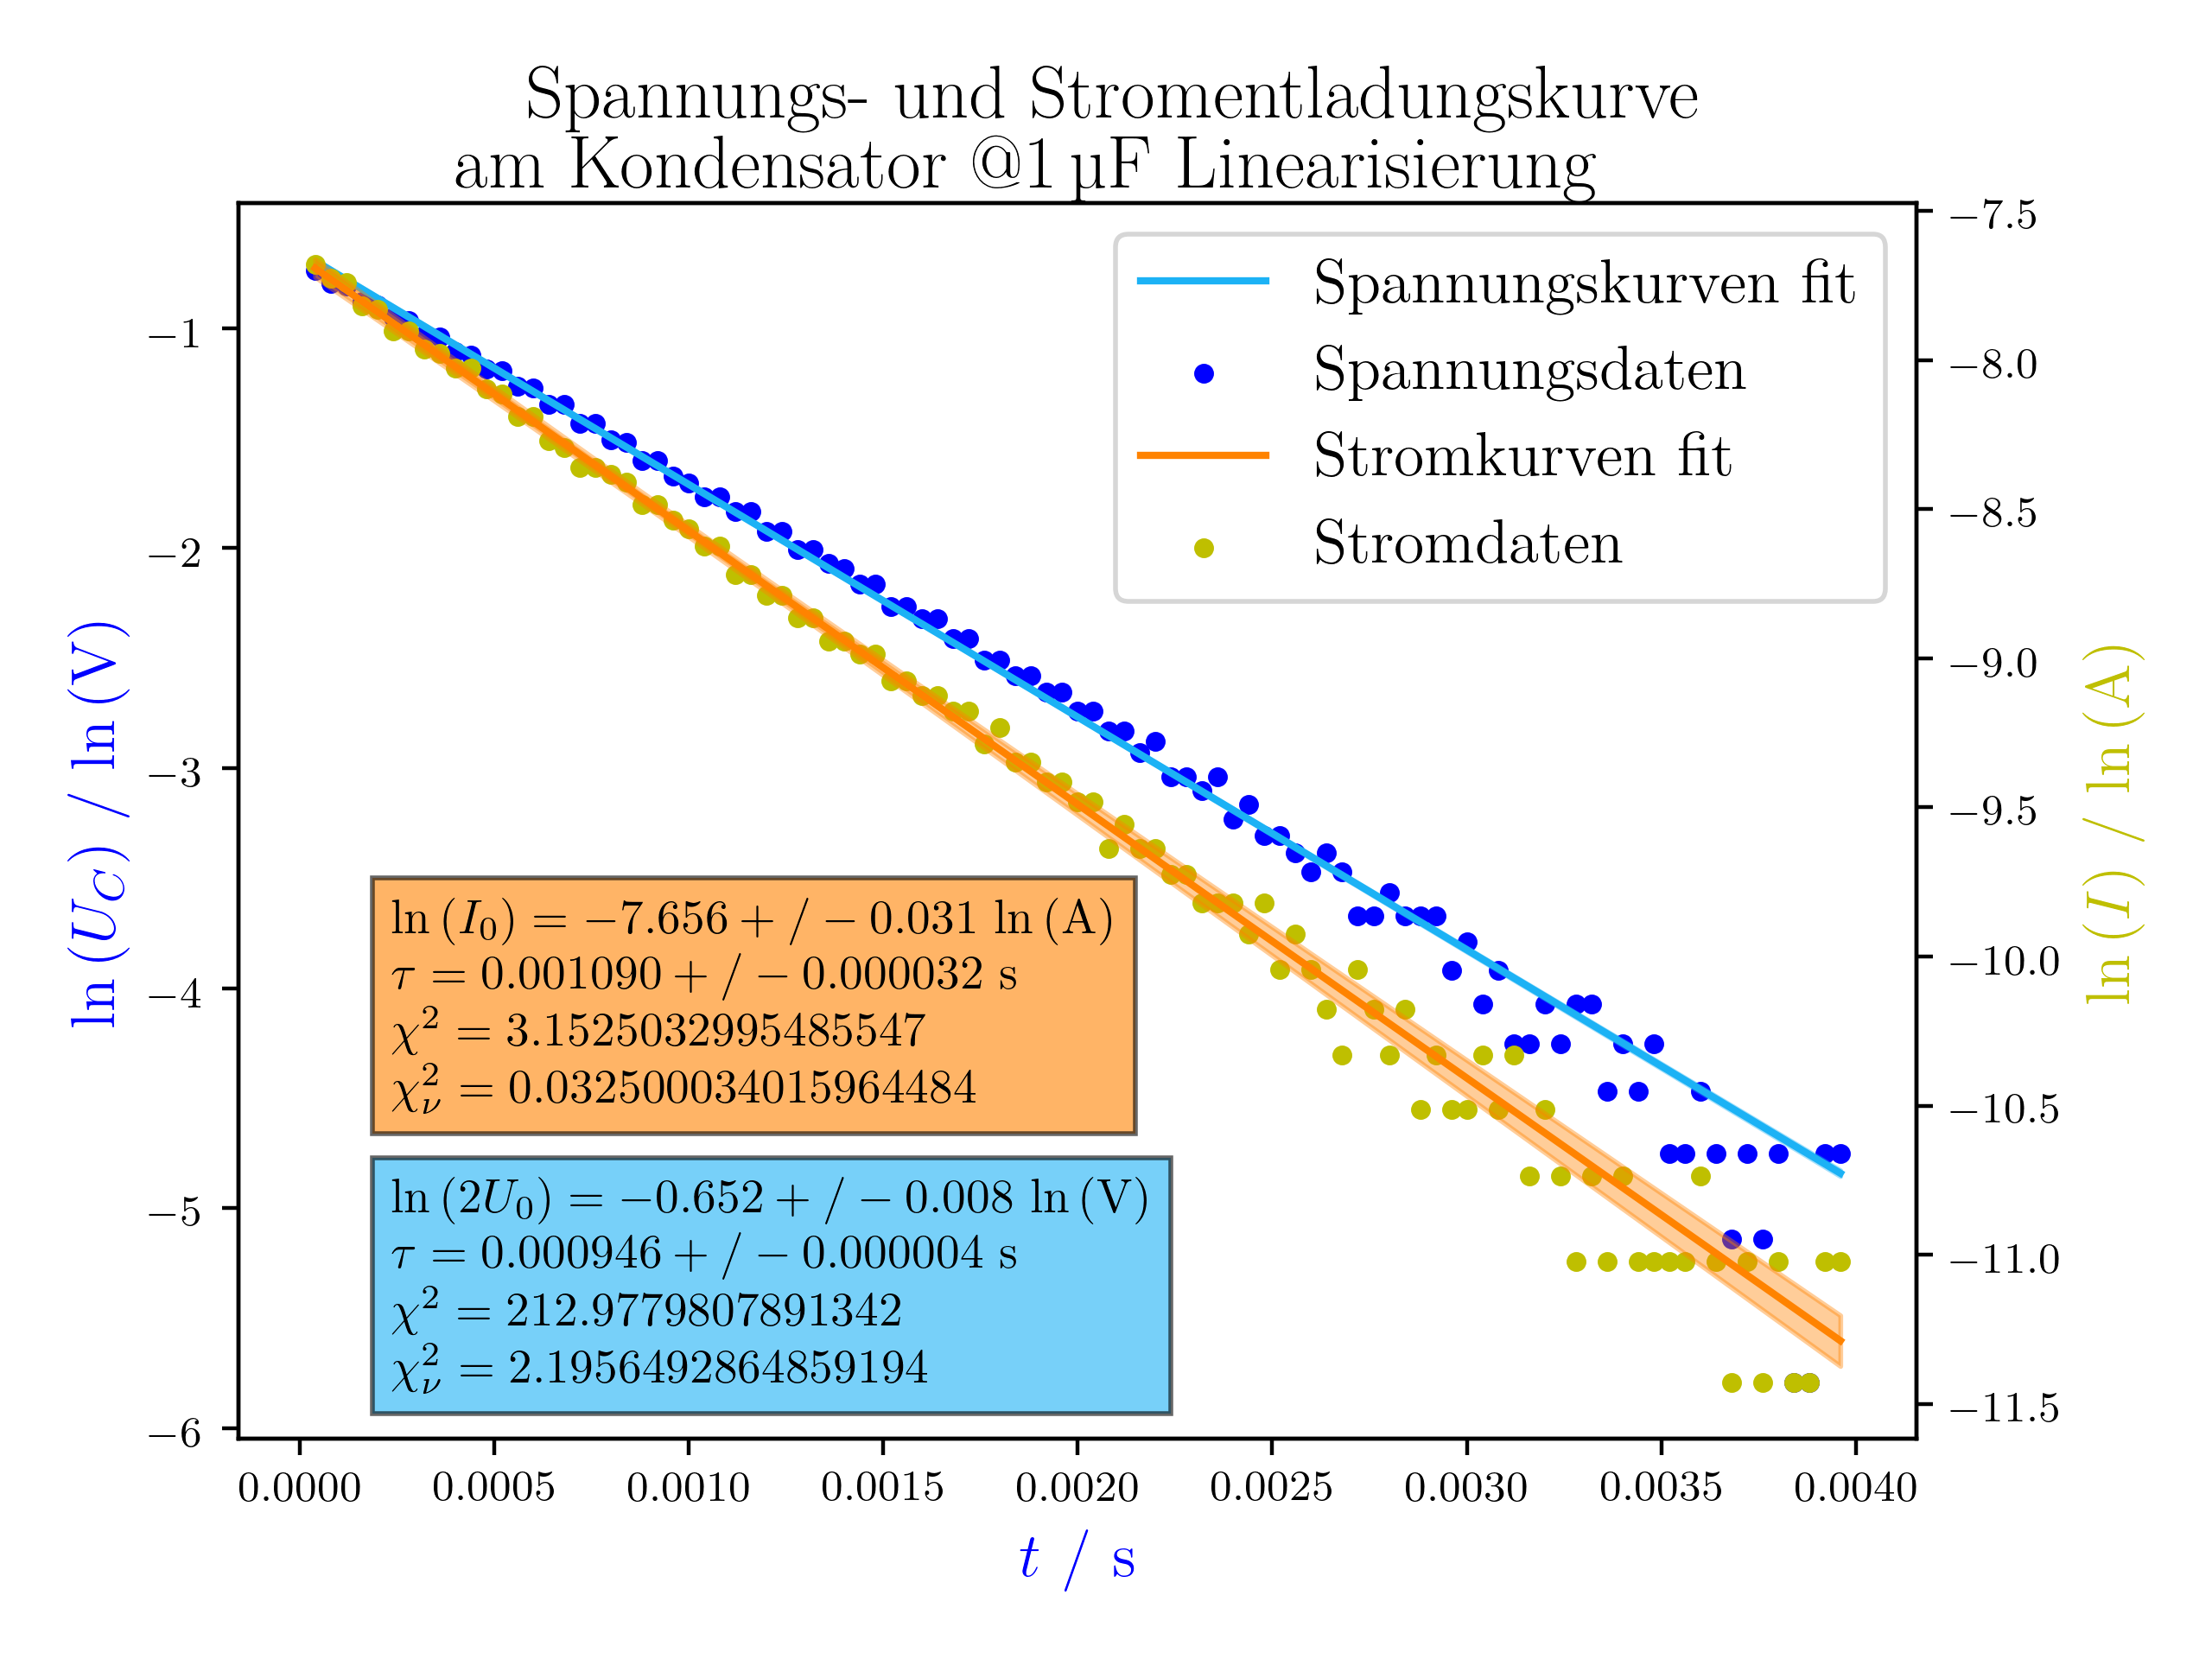
\includegraphics[width=\textwidth]{figures/entladekurve_linear}
	\end{minipage}
	\begin{minipage}{0.49\textwidth}
		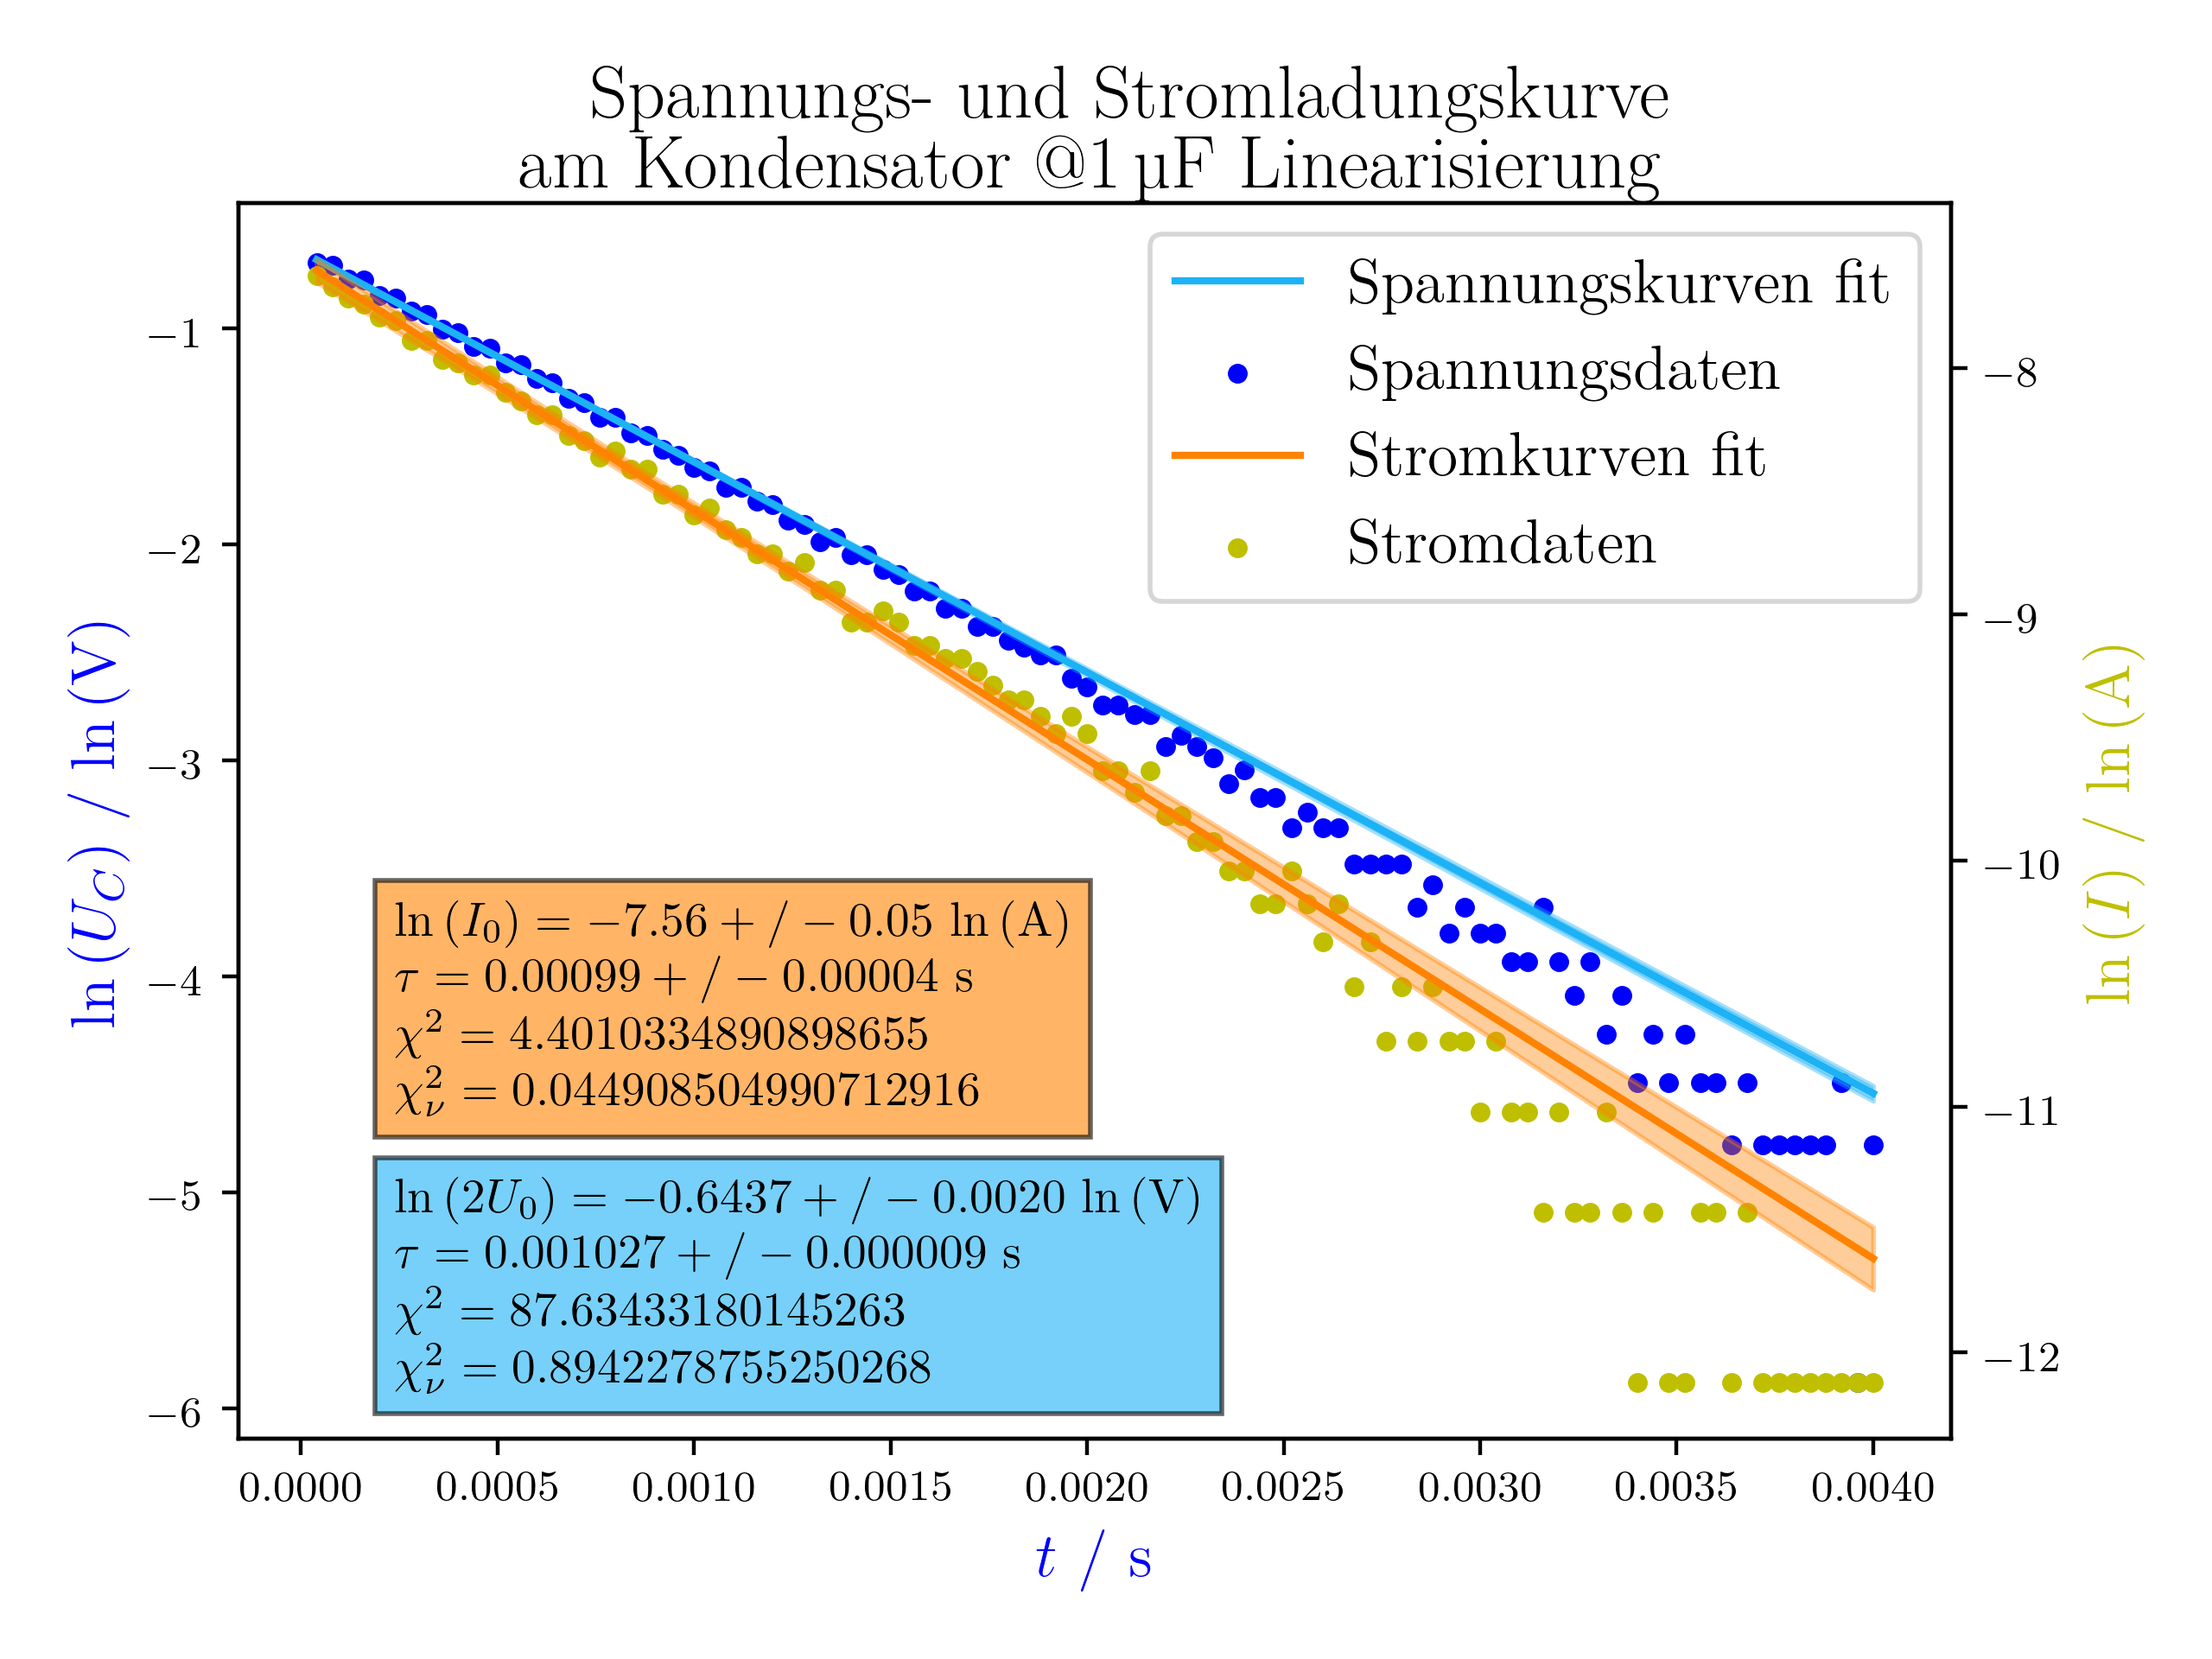
\includegraphics[width=\textwidth]{figures/ladekurve_linear}
	\end{minipage}
	\caption{Dies ist der linearisierte Fit der Strom- (gelb) und Spannungs-
		(blau) Ladekurve und Entladekurve eines RC Kreises mit einem Widerstand R
		von \SI{1000(100)}{\ohm} und einer Kapazität C von
		\SI{1.0(1)}{\micro\farad}. Die Daten sind aus
		\autoref{fig:rechteckschw_groß} entnommen worden}
	\label{fig:linear_fit}
\end{figure}

\newpage

\section{Diskussion}\label{disk}

\subsection{Kennenlernen des Kathodenstrahloszilloskops}

Aufgrund leicht aus dem Gleichgewicht bring-baren Einstellung der Frequenzen
ist es relativ schwierig einen perfekten Kreis abzubilden, der nicht rotiert
und somit die Frequenzen aufeinander abzustimmen. Anhand der
Rotationsgeschwindigkeit kann die Schwebungsfrequenz bestimmt werden, welche
der Differenz der zwei Frequenzen entspricht.

Bei der Erzeugung der Knotenpunkte fällt diese Einstellung leichter, weil die
Einstellung der Punkte auf die Nulllinie, dem Menschen leichter fällt.

\subsection{Serienschaltung aus ohm´schen Widerstand und Kapazität}

% die auswertungsmethoden halbwertszeit, linearisierung, linearfit
Es ist klar ersichtlich das alle erhaltenen Werte aus den Fits mit dem theoretischen Wert von

\begin{equation}
	\tau_{\text{theo}} = RC = \SI{1000(100)}{\ohm} \; \SI{1.0(1)}{\micro\farad} = \SI{1.0(2)}{\ms}
	\label{eq:tautheo}
\end{equation}

größenordnungsmäßig übereinstimmen und in dessen Fehlerintervall
enthalten sind. Es ist jedoch anzumerken, dass das Linearisieren der Daten
hier nicht die beste Strategie ist, da die Auflösung des Oszilloskop zu gering
ist um niedrige Potenzen ($10^{-5}$ und niedriger) akkurat im linearisierten
Datensatz darzustellen.

Es gäbe noch eine dritte Methode die Zerfallskonstante zu bestimmen indem einfach die
Halbwertszeit gemessen wird. Da ``Matplotlib`` die Funktion auf eigenen
Achsen auf Fullscale zeichnet, die gleiche Zeitachse teilen und sie die gleiche
Zerfallskonstante in sich tragen, ist der Schnittpunkt der beiden Kurven gleich
der Hälfte des Anfangswerts. Somit ist der Wert an der x-Achsen-Stelle des
Schnittpunkts gleich der Halbwertszeit, welche so abgelesen werden kann. Damit kann $\tau$ auch
bestimmt werden indem $\tau = \frac{T_{1/2}}{ln{2}}$. Dies wurde auch per Hand
durchgeführt, lieferte aber nicht so überzeugende Werte weshalb entschieden wurde, diese nicht weiterzuverfolgen.

Ein Verbesserungsvorschlag wäre anstatt nur einen Wert mehrere Halbwertszeiten
computerunterstützt auszurechnen wodurch sich die Unsicherheit ein bisschen
bessern würde. Jedoch würde so auch das Problem mit der Auflösung
des Oszilloskops nicht umgangen werden.
%probleme programm



\subsection{Serienschwingkreis}

Um den Schwingfall zu erzeugen, muss folgender Wert möglichst negativ gebracht werden.

\begin{equation}
	\label{eq:schwingen}
	R^2 C - 4L < 0
\end{equation}

Weiters muss der Dämpfungsfaktor

\begin{equation}
	\label{eq:dampfung}
	\delta = \frac{R}{2L}
\end{equation}

möglichst minimiert werden, damit die Schwingung so lange wie möglich stattfinden kann.

\vspace{2mm}

Grundsätzlich hätten diese Werte nur durch das Einschieben von Eisenkernen
variiert werden sollen. Durch Erhöhen der Induktivität verhalten sich obige
Gleichungen wie gewünscht, indem \autoref{eq:schwingen} negativer und
\autoref{eq:dampfung} kleiner wird.

Um den Kriechfall noch weiter zu verbessern, wurden folgende Änderungen
vorgenommen.

Zunächst wird der Widerstand verringert, indem dieser halbiert wird, wodurch
sich folgende Grafik am Oszilloskop ergibt.

\begin{figure}[H]
	\begin{center}
		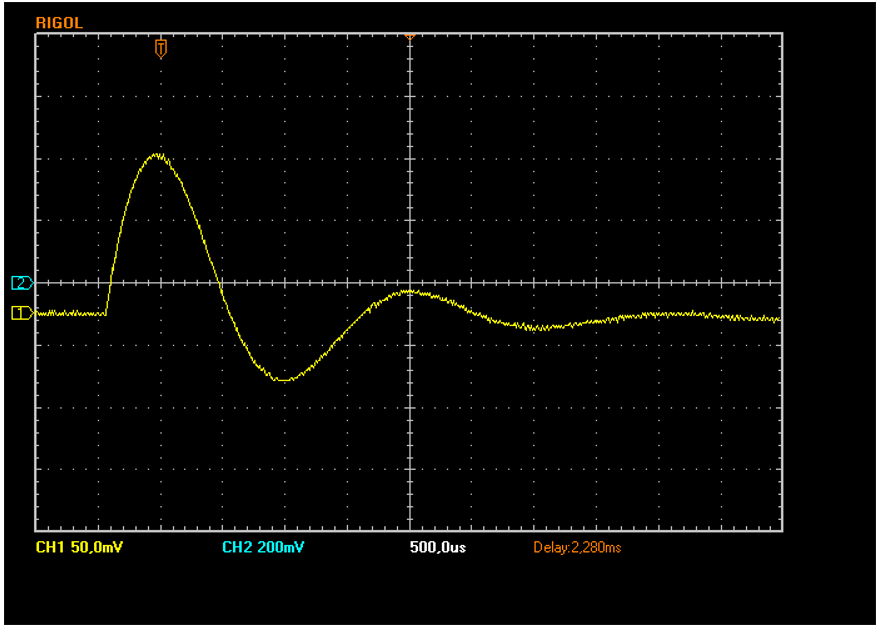
\includegraphics[width=0.7\textwidth]{Bild_versuch3_c_100}
	\end{center}
	\caption{Aufgezeichnetes Signal des Schwingfalls bei einer Anpassung des
		Widerstands auf \SI{100(10)}{\ohm}}
	\label{fig:schwingfall_100}
\end{figure}


Um nun eine noch stärkere Schwingung zu erzeugen werden 2 weitere Spulen mit
Eisenkern in die Schaltung mittels Serienschaltung integriert, wodurch sich
schließlich folgender Graph ergibt.

\begin{figure}[H]
	\begin{center}
		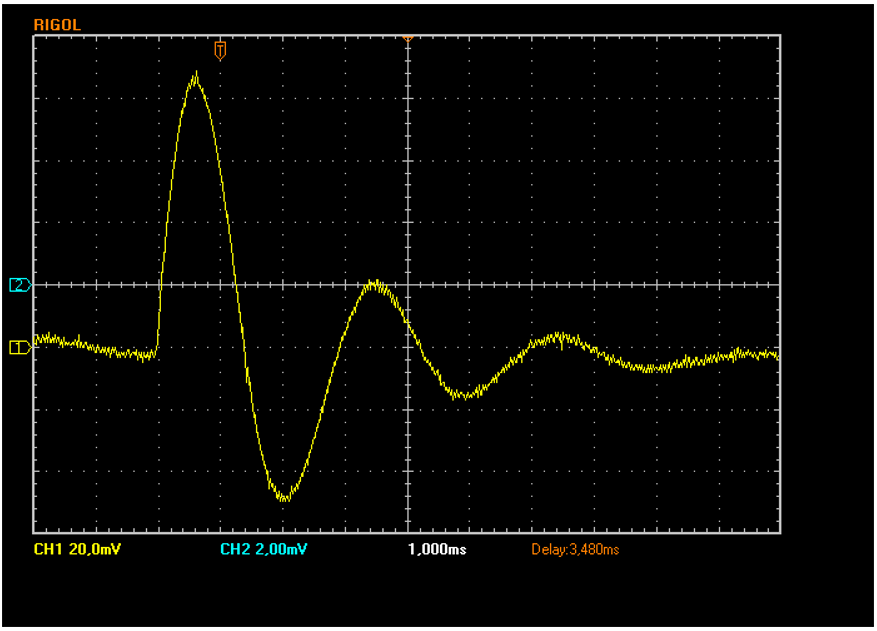
\includegraphics[width=0.7\textwidth]{Bild_versuch3_c_100_4}
	\end{center}
	\caption{Aufgezeichnetes Signal des Schwingfalls bei einer Anpassung des
		Widerstands auf \SI{100(10)}{\ohm} und der Verwendung von 4 Spulen}
	\label{fig:schwingfall_100_4}
\end{figure}

Betrachtet man nun die obigen Graphen ist ersichtlich, dass eine deutlich
größere Schwingung vorliegt, was sich auch mit den zuvor aufgestellten
Gleichungen deckt.


\newpage

\section{Zusammenfassung}

Mithilfe des Kathodenstrahloszilloskops konnten verschiedene ``Lissajou
Figuren`` erzeugt werden, wie beispielsweise in \autoref{fig:lissajou}
ersichtlich. Anhand deren Formen und Ausrichtungen können Aussagen über die
Frequenz- und Amplitudenverhältnisse getroffen werden.

\vspace{2mm}

%2
Beim Sinussignal ist, wie erwartet eine Phasenverschiebung zwischen Strom und
Spannung entstanden. Wie anhand \autoref{fig:sinusschw} ersichtlich ist, geht
beim Kondensator der Strom vor.

Weiters wurde das Entlade und Lade verhalten
eines Kondensators untersucht indem die gemessen Daten an einen
Exponentialfunktion gefittet wurden, um die Zerfallskonstante zu bestimmen. Zusätzlich
wurden die Spannnungs- und Stromdaten linearisiert und an linearen Funktionen
gefittet, welche auch im Unsicherheitsintervall des theoretischen Werts
liegen.

Hier werden nochmals alle erhaltenen Werte für die mittlere Lebensdauer mit
dem theoretischen Wert gegenübergestellt.

\begin{table}[H]
	\caption{Dies ist die Vergleichstabelle aller erhaltenen Werte für die mittlere
		Lebensdauer $\tau$ und deren multiplikativen Inversen der Zerfallskonstante $\lambda$}
	\label{tab:ergebniszerfallskonstante}
	\begin{center}
		\begin{tabular}[c]{l|c|c|c|c}
			\hline
			\multicolumn{1}{c|}{\textbf{}}                &
			\multicolumn{1}{c|}{$\tau$ / \si{\ms}}        &
			\multicolumn{1}{c|}{$\Delta \tau$ / \si{\ms}} &
			\multicolumn{1}{c|}{$\lambda$ / \si{\Hz}}     &
			\multicolumn{1}{c}{$\Delta \lambda$ / \si{\Hz}}                            \\
			\hline
			theo.                                         & 1.0   & 0.2   & 1000 & 200 \\
			lin. Laden Strom                              & 0.99  & 0.04  & 1010 & 50  \\
			lin. Laden Spannung                           & 1.027 & 0.009 & 974  & 9   \\
			lin. Entladen Strom                           & 1.09  & 0.04  & 920  & 40  \\
			lin. Entladen Spannung                        & 0.946 & 0.004 & 1046 & 5   \\
			exp. Laden Strom                              & 0.95  & 0.04  & 1050 & 50  \\
			exp. Laden Spannung                           & 1.028 & 0.008 & 973  & 8   \\
			exp. Entladen Strom                           & 0.96  & 0.03  & 1040 & 40  \\
			exp. Entladen Spannung                        & 0.896 & 0.003 & 1116 & 4   \\
			\hline
		\end{tabular}
	\end{center}
\end{table}

\vspace{2mm}

Die 3 Schwingfälle konnten durch Variation der Eisenkerne gezeigt werden.

\section{Anmerkungen}

Die ersten 3 Kapitel, sowie die dazugehörigen Abbildungen, wurden nicht von den
Autoren persönlich erstellt, sondern sind schon im Zuge der Aufgabenstellung,
in Form einer PDF, bereitgestellt und davon entnommen worden. \cite{vorlageoszi}


\newpage

%\bibliographystyle{unsrt}
%\bibliography{citations}
\printbibliography
\listoffigures
\listoftables
\end{document}
